%%% DO NOT EDIT the .tex file directly since it is generated from the .Rnw
%%% sources.
%\VignetteEngine{knitr::knitr}
%\VignetteIndexEntry{irace package: User Guide}
%\VignetteDepends{knitr}
%\VignetteCompiler{knitr}
%\VignetteEngine{knitr::knitr}
\RequirePackage[dvipsnames]{xcolor}
\documentclass[a4paper,english]{article}\usepackage[]{graphicx}\usepackage[]{color}
%% maxwidth is the original width if it is less than linewidth
%% otherwise use linewidth (to make sure the graphics do not exceed the margin)
\makeatletter
\def\maxwidth{ %
  \ifdim\Gin@nat@width>\linewidth
    \linewidth
  \else
    \Gin@nat@width
  \fi
}
\makeatother

\definecolor{fgcolor}{rgb}{0.345, 0.345, 0.345}
\newcommand{\hlnum}[1]{\textcolor[rgb]{0.686,0.059,0.569}{#1}}%
\newcommand{\hlstr}[1]{\textcolor[rgb]{0.192,0.494,0.8}{#1}}%
\newcommand{\hlcom}[1]{\textcolor[rgb]{0.678,0.584,0.686}{\textit{#1}}}%
\newcommand{\hlopt}[1]{\textcolor[rgb]{0,0,0}{#1}}%
\newcommand{\hlstd}[1]{\textcolor[rgb]{0.345,0.345,0.345}{#1}}%
\newcommand{\hlkwa}[1]{\textcolor[rgb]{0.161,0.373,0.58}{\textbf{#1}}}%
\newcommand{\hlkwb}[1]{\textcolor[rgb]{0.69,0.353,0.396}{#1}}%
\newcommand{\hlkwc}[1]{\textcolor[rgb]{0.333,0.667,0.333}{#1}}%
\newcommand{\hlkwd}[1]{\textcolor[rgb]{0.737,0.353,0.396}{\textbf{#1}}}%

\usepackage{framed}
\makeatletter
\newenvironment{kframe}{%
 \def\at@end@of@kframe{}%
 \ifinner\ifhmode%
  \def\at@end@of@kframe{\end{minipage}}%
  \begin{minipage}{\columnwidth}%
 \fi\fi%
 \def\FrameCommand##1{\hskip\@totalleftmargin \hskip-\fboxsep
 \colorbox{shadecolor}{##1}\hskip-\fboxsep
     % There is no \\@totalrightmargin, so:
     \hskip-\linewidth \hskip-\@totalleftmargin \hskip\columnwidth}%
 \MakeFramed {\advance\hsize-\width
   \@totalleftmargin\z@ \linewidth\hsize
   \@setminipage}}%
 {\par\unskip\endMakeFramed%
 \at@end@of@kframe}
\makeatother

\definecolor{shadecolor}{rgb}{.97, .97, .97}
\definecolor{messagecolor}{rgb}{0, 0, 0}
\definecolor{warningcolor}{rgb}{1, 0, 1}
\definecolor{errorcolor}{rgb}{1, 0, 0}
\newenvironment{knitrout}{}{} % an empty environment to be redefined in TeX

\usepackage{alltt}
\usepackage[a4paper]{geometry} % It saves some pages
\usepackage[utf8]{inputenc}
\usepackage[T1]{fontenc}
\usepackage[english]{babel}
\usepackage{ifthen}
\newboolean{Release}
\setboolean{Release}{false}
%\setboolean{Release}{true}
\usepackage{calc}
\usepackage{algorithm,algorithmic}
\usepackage{booktabs}
\usepackage{tabularx}
\usepackage{xspace}
\usepackage{amsmath,amssymb}
\usepackage{relsize}
\usepackage{fancyvrb}
\usepackage[hyphens]{url}
\usepackage{hyperref}
\usepackage[numbers]{natbib}
\usepackage[nottoc]{tocbibind}
%% For autoref
\hypersetup{
    colorlinks,
    linkcolor={red!50!black},
    citecolor={blue!50!black},
    urlcolor={blue!70!black}
}
\addto\extrasenglish{%
\def\sectionautorefname{Section}
\let\subsectionautorefname\sectionautorefname
\let\subsubsectionautorefname\sectionautorefname
}
\usepackage[titletoc, title]{appendix}
% Fix use with \autoref
\newcommand*{\Appendixautorefname}{Appendix}
\usepackage{tocloft}
\setlength{\cftsubsecnumwidth}{3em}% Set length of number width in ToC for \subsection
\usepackage[inline]{enumitem}
\setlist[enumerate]{leftmargin=*,widest=00}
\setlist[itemize]{leftmargin=1.5em}

%% FIXME: listing is very limited, we should use 'minted'
\usepackage{listings}
\lstdefinestyle{BashInputStyle}{
  language=bash,%
  basicstyle=\ttfamily,%
  numbers=none,%
  frame=tb,%
  rulecolor=\color{lightgray},
%  framesep=1ex,
  framexleftmargin=1ex,
  columns=fullflexible,%
  backgroundcolor=\color{yellow!05},%
  linewidth=\linewidth,%
 % xleftmargin=1\linewidth,%
  identifierstyle=\color{darkgray},%
  keywordstyle=\color{darkgray},%
  keywordstyle={[2]\color{Cyan}},%
  keywordstyle={[3]\color{olive}},%
  stringstyle=\color{MidnightBlue},%
  commentstyle=\color{RedOrange},%
  morestring=[b]',%
}

\DefineVerbatimEnvironment{Code}{Verbatim}{}
\DefineVerbatimEnvironment{CodeInput}{Verbatim}{fontshape=rm}
\DefineVerbatimEnvironment{CodeOutput}{Verbatim}{}
\newenvironment{CodeChunk}{}{}

\newcommand{\IRACEHOME}[1]{\hyperlink{irace_home}{\path{$IRACE_HOME}}\path{#1}}

\providecommand{\keywords}[1]{\textbf{\textit{Index terms---}} #1}

% Simple font selection is not good enough.  For example, |\texttt{--}|
% gives `\texttt{--}', i.e., an endash in typewriter font.  Hence, we
% need to turn off ligatures, which currently only happens for commands
% |\code| and |\samp| and the ones derived from them.  Hyphenation is
% another issue; it should really be turned off inside |\samp|.  And
% most importantly, \LaTeX{} special characters are a nightmare.  E.g.,
% one needs |\~{}| to produce a tilde in a file name marked by |\file|.
% Perhaps a few years ago, most users would have agreed that this may be
% unfortunate but should not be changed to ensure consistency.  But with
% the advent of the WWW and the need for getting `|~|' and `|#|' into
% URLs, commands which only treat the escape and grouping characters
% specially have gained acceptance
\makeatletter
\DeclareRobustCommand\code{\bgroup\@makeother\_\@makeother\~\@makeother\$\@noligs\@codex}
\def\@codex#1{\texorpdfstring%
{{\normalfont\ttfamily\hyphenchar\font=-1 #1}}%
{#1}\egroup}
\makeatother

\let\proglang=\textsf
\newcommand{\pkg}[1]{{\fontseries{b}\selectfont #1}}
\newcommand{\aR}{\proglang{R}\xspace}
\newcommand{\eg}{e.g.,\xspace}
\newcommand{\SoftwarePackage}{\pkg}
\newcommand{\ACOTSP}{\SoftwarePackage{ACOTSP}\xspace}

%% How to use this command:
% Parameter with one short switch: \defparameter[short]{paramName}{long}{default}
% Parameter without short switch:  \defparameter{paramName}{long}{default}
% Parameter without switch:  \defparameter{paramName}{}{default}
\newcommand{\defparameter}[4][]{%
\item[\code{#2}]\hypertarget{opt:#2}{} ~~ %
\ifthenelse{\equal{#3}{}}{}{%
  \emph{flag:} %
  \ifthenelse{\equal{#1}{}}{}{%
    \code{-#1}~~~\emph{or}~~~}%
  \code{-{}-#3} ~~ }%
\emph{default:}~\texttt{#4} \\
}
\newcommand{\parameter}[1]{\hyperlink{opt:#1}{\code{#1}}}


\newcommand{\irace}{\pkg{irace}\xspace}
\newcommand{\Irace}{\pkg{Irace}\xspace}
\newcommand{\race}{\pkg{race}\xspace}
\newcommand{\FRACE}{\text{F-Race}\xspace}
\newcommand{\IFRACE}{\text{I/F-Race}\xspace}
\newcommand{\iraceversion}{2.3}

\newcommand{\Niter}{\ensuremath{N^\text{iter}}\xspace}
\newcommand{\Nparam}{\ensuremath{{N^\text{param}}}\xspace}
\newcommand{\iter}{\ensuremath{j}\xspace}
\newcommand{\Budget}{\ensuremath{B}\xspace}
\newcommand{\Budgetj}{\ensuremath{\Budget_{\iter}}\xspace}
\newcommand{\Bused}{\ensuremath{\Budget_\text{used}}\xspace}
\newcommand{\Ncand}[1][]{\ensuremath{N_{#1}}\xspace}
\newcommand{\Mui}{\ensuremath{\mu_{\iter}}\xspace}
\newcommand{\Nmin}{\ensuremath{N^\text{min}}\xspace}
\newcommand{\Nsurv}{\ensuremath{N^\text{surv}}\xspace}
\newcommand{\Nelite}{\ensuremath{N^\text{elite}}\xspace}
\newcommand{\Nnew}{\ensuremath{N^\text{new}}\xspace}

\ifthenelse {\boolean{Release}}{%
\newcommand{\MANUEL}[1]{}
\newcommand{\LESLIE}[1]{}
\newcommand{\THOMAS}[1]{}
}{%
\newcommand{\MANUEL}[1]{{\footnotesize\noindent\textbf{\color{red}[~MANUEL: #1~]}}}
\newcommand{\LESLIE}[1]{\footnote{\noindent\textbf{[ LESLIE: #1 ]}}}
\newcommand{\THOMAS}[1]{\footnote{\noindent\textbf{[ THOMAS: #1 ]}}}
}
\newcommand{\hide}[1]{}

\usepackage{tcolorbox}
\newcommand{\infoicon}{%
\parbox[c]{0.75cm}{
\includegraphics[keepaspectratio=true,width=0.75cm]{light-bulb-icon}}%
\hspace{1em}}
\newcommand{\warningicon}{%
\parbox[c]{0.75cm}{
\includegraphics[keepaspectratio=true,width=0.75cm]{Warning-icon}}%
\hspace{1em}}

\definecolor{LightGray}{RGB}{193,193,193}
\definecolor{LightYellow}{RGB}{253,247,172}

\newlength\macroiconwidth
\newenvironment{xwarningbox}{%
\setlength{\fboxrule}{3.0\fboxrule}%
\setlength{\fboxsep}{0\fboxsep}%
\begin{tcolorbox}[colback=LightYellow,colframe=LightGray,boxrule=\fboxrule,boxsep=\fboxsep]%
\infoicon%
\settowidth{\macroiconwidth}{\infoicon}%
\begin{minipage}[c]{\columnwidth - \macroiconwidth - 2.0\fboxrule - 2.0\fboxsep}
\raggedright\footnotesize
%
}{%
\end{minipage}
\end{tcolorbox}
%
}
\IfFileExists{upquote.sty}{\usepackage{upquote}}{}
\begin{document}



\author{Manuel L\'opez-Ib\'a\~nez, Leslie P\'erez C\'aceres, J\'er\'emie Dubois-Lacoste,\\
  Thomas St\"utzle and Mauro Birattari
\\IRIDIA, CoDE, Universit\'e Libre de Bruxelles, Brussels, Belgium}

\title{The \irace Package: User Guide}
\date{Version \iraceversion, \today}
%\keywords{automatic
%  algorithm configuration, racing, parameter tuning, \aR}

\maketitle

\tableofcontents

%Load files needed for examples

\newpage

%%
%%
%%
%% General info
%%
%%
%%
\section{General information}
\MANUEL{Some things could be taken from the intro of the irace paper and reformulated.}
\MANUEL{It would be good to mention that not only opt algorithms can be configured with irace, we say this in the paper.}

\subsection{Background}
\MANUEL{I would add a paragraph defining what is irace (a bit longer than the abstract above) and references to the literature so people can find more info. The first reference should be the irace TR.} \LESLIE{Here i guess we should say why tune an algorithm is a good idea, and why using irace is a better one.}
The \irace package implements an \emph{iterated racing} procedure,
which is an extension of Iterated F-race (\IFRACE)~\cite{BirYuaBal2010:emaoa}.  The main use of
\irace is the automatic configuration of optimization and decision algorithms,
that is, finding the most appropriate settings of an algorithm given a 
set of instances of a problem. However, it may also be useful for 
configuring other types of algorithms when performance depends on 
the used parameter settings. It builds upon the \pkg{race} package 
by Birattari and it is implemented in \aR. The \irace
package is available from CRAN. More information about \irace is
available at \url{http://iridia.ulb.ac.be/irace}.

\subsection{Version}
The current version of the \irace package is \iraceversion. Previous
versions of the package can be found in the CRAN website.
\begin{center}
\url{https://cran.r-project.org/web/packages/irace/}
\end{center}
%
\begin{xwarningbox}
  Versions of \irace before 2.0 are not compatible with the file formats
  detailed in this document.
\end{xwarningbox}

The algorithm underlying the current version of \irace and its motivation are
described by \citet{LopDubPerStuBir2016irace}. Details of the implementation
before version 2.0 can be found in a previous technical
report~\cite{LopDubStu2011irace}.


\subsection{License}

The \irace package is Copyright \copyright{} 2016 and distributed under the GNU General Public
License version 3.0 (\url{http://www.gnu.org/licenses/gpl-3.0.en.html}).
The \irace package is free software (software libre): you can redistribute it and/or modify it under the terms
of the GNU General Public License as published by the Free Software Foundation,
either version 3 of the License, or (at your option) any later version.

The \irace package is distributed in the hope that it will be useful, but
WITHOUT ANY WARRANTY; without even the implied warranty of MERCHANTABILITY or
FITNESS FOR A PARTICULAR PURPOSE.

Please be aware that the fact that this program is released as Free Software
does not excuse you from scientific propriety, which obligates you to give
appropriate credit! If you write a scientific paper describing research that
made substantive use of this program, it is your obligation as a scientist to
(a) mention the fashion in which this software was used in the Methods section;
(b) mention the algorithm in the References section. The appropriate citation
is:

\begin{itemize}[leftmargin=3em]
\item[] Manuel López-Ibáñez, Jérémie Dubois-Lacoste, Leslie Pérez Cáceres,
  Thomas Stützle, and Mauro Birattari. The \irace package: Iterated Racing for
  Automatic Algorithm Configuration. \emph{Operations Research Perspectives}, 3:43--58, 2016.
  doi:~\href{http://dx.doi.org/10.1016/j.orp.2016.09.002}{10.1016/j.orp.2016.09.002}

\end{itemize}

\section{Before starting}
\MANUEL{I think this could be a bit more detailed by defining what is a parameter, a configuration, an instance, etc. but ok for now.}

The \irace package provides an automatic configuration tool for
 tuning optimization algorithms, that is, automatically finding good configurations for the parameters values
of a (target) algorithm saving the effort that normally requires manual
tuning.

\begin{figure}[t]
  \centering
  \includegraphics[width=0.6\textwidth]{irace-scheme}
  \caption{Scheme of \irace flow of information.}
\label{fig:irace-scheme}
\end{figure}

Figure~\ref{fig:irace-scheme} gives a general scheme of how \irace works.
\Irace receives as input a \emph{parameter space definition} corresponding to the
parameters of the target algorithm that will be tuned, a set of \emph{instances}
for which the parameters must be tuned for and a set of options for \irace that define the \emph{configuration scenario}. Then, \irace searches in the parameter search space for good performing algorithm
configurations by executing the target algorithm on different instances and
with different parameter configurations. A \parameter{targetRunner} must be provided to execute the target algorithm with a
specific parameter configuration ($\theta$) and instance ($i$). The \parameter{targetRunner} function (or program) acts
as an interface between the execution of the target algorithm and \irace: It
receives the instance and configuration as arguments and must return the
evaluation of the execution of the target algorithm.

The following user guide contains guidelines for installing \irace, defining
configuration scenarios, and using \irace to automatically configure your
algorithms.

%%
%%
%%
%% Installation
%%
%%
%%

\section{Installation}

\subsection{System requirements}
\begin{itemize}
\item \aR ($\text{version} \geq 2.15$) is required for running irace, but you don't
  need to know the \aR language to use it.  \aR is freely available and you can
  download it from the \aR project website
  (\url{https://www.r-project.org}). See \autoref{sec:installation} for a
  quick installation guide of \aR.

\item For GNU/Linux and OS X, the command-line executables \code{irace} and
  \code{parallel-irace} require GNU Bash. There is also a \code{irace.bat} for
  Windows. Individual examples may require additional software.
\end{itemize}

\subsection{\irace installation} \label{sec:irace install}

The \irace package can be installed automatically within \aR or
by manual download and installation. We advise to use the automatic
installation unless particular circumstances do not allow it. The instructions
to install \irace with the two mentioned methods are the following:

\subsubsection[Install automatically within R]{Install automatically within \aR{}}

Execute the following line in the \aR console to install the package:
\begin{knitrout}
\definecolor{shadecolor}{rgb}{0.969, 0.969, 0.969}\color{fgcolor}\begin{kframe}
\begin{alltt}
\hlkwd{install.packages}\hlstd{(}\hlstr{"irace"}\hlstd{)}
\end{alltt}
\end{kframe}
\end{knitrout}
Select a mirror close to your location, and test the installation in the \aR console with:
\begin{knitrout}
\definecolor{shadecolor}{rgb}{0.969, 0.969, 0.969}\color{fgcolor}\begin{kframe}
\begin{alltt}
\hlkwd{library}\hlstd{(}\hlstr{"irace"}\hlstd{)}
\hlkwd{q}\hlstd{()} \hlcom{# To exit R}
\end{alltt}
\end{kframe}
\end{knitrout}

Alternatively, within the \aR graphical interface, you may use
the \code{Packages and data->Package installer} menu on OS X or the \code{Packages} menu on Windows.

\subsubsection{Manual download and installation}

From the \irace package CRAN website
(\url{https://cran.r-project.org/package=irace}), download one of the three
versions available depending on your operating system:
\begin{itemize}
\item \code{irace_\iraceversion.tar.gz} (Unix/BSD/GNU/Linux)
\item \code{irace_\iraceversion.tgz} (OS X)
\item \code{irace_\iraceversion.zip} (Windows)
\end{itemize}

To install the package on GNU/Linux and OS X, you must execute the following
command at the shell:
%
\begin{lstlisting}[style=BashInputStyle]
# Replace <package> with the path to the downloaded file.
R CMD INSTALL <package>
\end{lstlisting}

To install the package on Windows, open \aR and execute the following line on
the \aR console:
%\LESLIE{Check that this actually works on internet says that  this: \code{Rscript -e "install.packages('foo.zip', repos = NULL)"} also works}

\begin{knitrout}
\definecolor{shadecolor}{rgb}{0.969, 0.969, 0.969}\color{fgcolor}\begin{kframe}
\begin{alltt}
\hlcom{# Replace <package> with the path to the downloaded file.}
\hlkwd{install.packages}\hlstd{(}\hlstr{"<package>"}\hlstd{,} \hlkwc{repos} \hlstd{=} \hlkwa{NULL}\hlstd{)}
\end{alltt}
\end{kframe}
\end{knitrout}

If the previous installation instructions fail because of insufficient
permissions and you do not have sufficient admin rights to install \irace
system-wide, then you need to force a local installation.

\subsubsection{Local installation}

Let's assume you wish to install \irace on a path denoted by
\code{<R_LIBS_USER>}, which is a filesystem path for which you have sufficient
rights. This directory \textbf{must} exist before attempting the
installation. Moreover, you must provide to \aR the path to this
library when loading the package. However, the latter can be avoided by adding
the path to the system variable \code{R_LIBS} or to the \aR internal variable
\code{.libPaths}, as we will see below.\footnote{%
   On Windows, see also
   \url{https://cran.r-project.org/bin/windows/base/rw-FAQ.html\#I-don_0027t-have-permission-to-write-to-the-R_002d3_002e3_002e1_005clibrary-directory}.}


On GNU/Linux or OS X, execute the following commands to install the
package on a local directory:

\begin{lstlisting}[style=BashInputStyle]
export R_LIBS_USER="<R_LIBS_USER>"
# Create R_LIBS_USER if it doesn't exist
mkdir $R_LIBS_USER
# Replace <package> with the path to the downloaded file.
R CMD INSTALL --library=$R_LIBS_USER <package>
# Tell R where to find R_LIBS_USER
export R_LIBS=${R_LIBS_USER}:${R_LIBS}
\end{lstlisting}

On Windows, you can install the package on a local directory by executing the
following lines in the \aR console:

\begin{knitrout}
\definecolor{shadecolor}{rgb}{0.969, 0.969, 0.969}\color{fgcolor}\begin{kframe}
\begin{alltt}
\hlcom{# Replace <package> with the path to the downloaded file.}
\hlcom{# Replace <R_LIBS_USER> with the path used for installation.}
\hlkwd{install.packages}\hlstd{(}\hlstr{"<package>"}\hlstd{,} \hlkwc{repos} \hlstd{=} \hlkwa{NULL}\hlstd{,} \hlkwc{lib} \hlstd{=} \hlstr{"<R_LIBS_USER>"}\hlstd{)}
\hlcom{# Tell R where to find R_LIBS_USER.}
\hlcom{# This must be executed for every new session.}
\hlkwd{.libPaths}\hlstd{(}\hlkwd{c}\hlstd{(}\hlstr{"<R_LIBS_USER>"}\hlstd{,} \hlkwd{.libPaths}\hlstd{()))}
\end{alltt}
\end{kframe}
\end{knitrout}

\subsubsection{Testing the installation and invoking irace}

Once \irace has been installed, load the package and test that the installation
was successful by opening an \aR console and executing:

\begin{knitrout}
\definecolor{shadecolor}{rgb}{0.969, 0.969, 0.969}\color{fgcolor}\begin{kframe}
\begin{alltt}
\hlcom{# Load the package}
\hlkwd{library}\hlstd{(}\hlstr{"irace"}\hlstd{)}
\hlcom{# Obtain the installation path}
\hlkwd{system.file}\hlstd{(}\hlkwc{package} \hlstd{=} \hlstr{"irace"}\hlstd{)}
\end{alltt}
\end{kframe}
\end{knitrout}

The last command must print out the filesystem path  where \irace is
installed.  In the remainder of this guide, the variable
\code{\$IRACE_HOME} is used to denote this path. When executing any provided
command that includes the \code{\$IRACE_HOME} variable do not forget to replace
this variable with the installation path of \irace.

On GNU/Linux or OS X, you can let the operating system know where to find \irace
by defining the \code{\$IRACE_HOME} variable and adding it to the system
\code{PATH}. Append the following commands to \path{~/.bash_profile}, \path{~/.bashrc} or
\path{~/.profile}:
%
%<<linux_irace_path1,engine='bash',eval=FALSE>>=
\begin{lstlisting}[style=BashInputStyle]
# Replace <IRACE_HOME> with the irace installation path
export IRACE_HOME=<IRACE_HOME>
export PATH=${IRACE_HOME}/bin/:$PATH
# Tell R where to find R_LIBS_USER
# Use the following line only if local installation was forced
export R_LIBS=${R_LIBS_USER}:${R_LIBS}
\end{lstlisting}
%@

Then, open a new terminal and launch \irace as follows:

%<<linux_irace_help,engine='bash',eval=FALSE>>=
\begin{lstlisting}[style=BashInputStyle]
irace --help
\end{lstlisting}
%@

On Windows, you need to add both \aR and the installation path of \irace to the
environment variable \code{PATH}. To edit the \code{PATH}, search for
``Environment variables'' in the control panel, edit \code{PATH} and add
a string similar to \path{C:\R_PATH\bin;C:\IRACE_HOME\bin} where \code{R_PATH}
is the installation path of \aR and \code{IRACE_HOME} is the installation path
of \irace. If \irace was installed locally, you also need to edit the
environment variable \code{R_LIBS} to add \code{R_LIBS_USER}. Then, open a new
terminal (run program \code{cmd.exe}) and launch \irace as:
%
%<<win_irace_help,engine='bash',eval=FALSE>>=
\begin{lstlisting}[style=BashInputStyle]
irace.bat --help
\end{lstlisting}
%@

Alternatively, you may directly invoke \irace from within the \aR
console by executing:
\begin{knitrout}
\definecolor{shadecolor}{rgb}{0.969, 0.969, 0.969}\color{fgcolor}\begin{kframe}
\begin{alltt}
\hlkwd{library}\hlstd{(}\hlstr{"irace"}\hlstd{)}
\hlkwd{irace.cmdline}\hlstd{(}\hlstr{"--help"}\hlstd{)}
\end{alltt}
\end{kframe}
\end{knitrout}


\section{Running irace}\label{sec:execution}

Before performing the tuning of your algorithm, it is necessary to define a
tuning scenario that will give \irace all the necessary information to optimize the
parameters of the algorithm. The tuning scenario is composed of the following elements:

\begin{enumerate}
\item Target algorithm parameter description (see \autoref{sec:target parameters}).
\item Target algorithm runner (see \autoref{sec:runner}).
\item Training instances list (see \autoref{sec:training})
\item \irace options (see \autoref{sec:irace options}).
\item \textit{Optional:} Initial configurations (see \autoref{sec:initial}).
\item \textit{Optional:} Forbidden configurations (see \autoref{sec:forbidden}).
\item \textit{Optional:} Target algorithm evaluator (see \autoref{sec:evaluator}).
\end{enumerate}

These scenario elements can be provided as plain text files
or as \aR objects. This user guide provides examples of both types,
but we advise the use of plain text files, which we consider the simpler
option.

For a step-by-step guide to create the scenario elements for your target algorithm
continue to \autoref{sec:step}. For an example execution of \irace using the
\ACOTSP scenario go to \autoref{sec:example}.

Once all the scenario elements are prepared you can execute \irace, either using the command-line wrappers provided by the package
 or directly from the \aR console:


\begin{itemize}
\item Execute \irace from the command-line as (on Windows, you should execute
  \code{irace.bat}):

%<<irace_cmd_exe0,engine='bash', eval=FALSE>>=
\begin{lstlisting}[style=BashInputStyle]
# $IRACE_HOME is the installation directory of irace.
$IRACE_HOME/bin/irace --scenario scenario.txt
\end{lstlisting}
%@

For this example we assume that the needed scenario files have been set
properly in the \code{scenario.txt} file using the options described in
\autoref{sec:irace options}. Most \irace options can be specified
in the command line or directly in the \code{scenario.txt} file.

\item Or execute \irace from the \aR console as:

\begin{knitrout}
\definecolor{shadecolor}{rgb}{0.969, 0.969, 0.969}\color{fgcolor}\begin{kframe}
\begin{alltt}
\hlkwd{library}\hlstd{(}\hlstr{"irace"}\hlstd{)}
\hlstd{parameters} \hlkwb{<-} \hlkwd{readParameters}\hlstd{(}\hlstr{"parameters.txt"}\hlstd{)}
\hlstd{scenario} \hlkwb{<-} \hlkwd{readScenario}\hlstd{(}\hlkwc{filename} \hlstd{=} \hlstr{"scenario.txt"}\hlstd{,}
                         \hlkwc{scenario} \hlstd{=} \hlkwd{defaultScenario}\hlstd{())}
\hlkwd{irace}\hlstd{(}\hlkwc{scenario} \hlstd{= scenario,} \hlkwc{parameters} \hlstd{= parameters)}
\end{alltt}
\end{kframe}
\end{knitrout}

\end{itemize}

The \irace executable provides an option (\code{--check}) to check that the scenario is
correctly defined. We recommend to perform a check every time
you create a new scenario. When performing the check, \irace will
verify that the scenario and parameter definitions are correct and
will test the execution of the target algorithm. To check your scenario
execute the following commands:

\begin{itemize}
\item From the command-line (on Windows, execute \code{irace.bat}):
  
%<<irace_check,engine='bash', eval=FALSE>>=
\begin{lstlisting}[style=BashInputStyle]
# $IRACE_HOME is the installation directory of irace.
$IRACE_HOME/bin/irace --scenario scenario.txt --check
\end{lstlisting}
%@

\item Or from the \aR console:

\begin{knitrout}
\definecolor{shadecolor}{rgb}{0.969, 0.969, 0.969}\color{fgcolor}\begin{kframe}
\begin{alltt}
\hlkwd{library}\hlstd{(}\hlstr{"irace"}\hlstd{)}
\hlstd{parameters} \hlkwb{<-} \hlkwd{readParameters}\hlstd{(}\hlstr{"parameters.txt"}\hlstd{)}
\hlstd{scenario} \hlkwb{<-} \hlkwd{readScenario}\hlstd{(}\hlkwc{filename} \hlstd{=} \hlstr{"scenario.txt"}\hlstd{,}
                         \hlkwc{scenario} \hlstd{=} \hlkwd{defaultScenario}\hlstd{())}
\hlkwd{checkIraceScenario}\hlstd{(}\hlkwc{scenario} \hlstd{= scenario,} \hlkwc{parameters} \hlstd{= parameters)}
\end{alltt}
\end{kframe}
\end{knitrout}

\end{itemize}

\subsection{Step-by-step setup guide}\label{sec:step}
This section provides a guide to setup a basic execution of \irace. The
template files provided in the package (\IRACEHOME{/templates}) will be
used as basis for creating your new scenario. Please follow carefully the
indications provided in each step and in the template files used; if you have
doubts check the the sections that describe each option in detail.

\begin{enumerate}[leftmargin=*]
\item Create a directory (\eg~\path{~/tuning/}) for the scenario setup. This directory will contain
all the files that describe the scenario. On GNU/Linux or OS X, you can do this as follows:
%<<dir1,engine='bash',eval=FALSE>>=
\begin{lstlisting}[style=BashInputStyle]
mkdir ~/tuning
cd ~/tuning
\end{lstlisting}
%@

\item Copy all the template files from the \IRACEHOME{/templates/}
directory to the scenario directory.
%<<copy1,engine='bash',eval=FALSE>>=
\begin{lstlisting}[style=BashInputStyle]
# $IRACE_HOME is the installation directory of irace.
cp $IRACE_HOME/templates/*.tmpl  ~/tuning/
\end{lstlisting}
%@

% Remember that \IRACEHOME{} is the path to the installation
% directory of \irace. It can be obtained in the \aR console with:
%
% <<irace_path,eval=FALSE, prompt=FALSE>>=
% library("irace")
% system.file(package = "irace")
% @

\item For each template in your tuning directory, remove the \code{.tmpl}
    suffix, and modify them following the next steps.

\item Define the target algorithm parameters to be tuned by following the
instructions in \code{parameters.txt}.  Available parameter types and other
guidelines can be found in \autoref{sec:target parameters}.


\item \textit{Optional}: Define the initial parameter configuration(s) of your
algorithm, which  allows you to provide good starting configurations (if you know
some) for the tuning. Follow the instructions in \code{configurations.txt} and set \parameter{configurationsFile}\code{="configurations.txt"} in \code{scenario.txt}. More
information in \autoref{sec:initial}. If you do not need to
define initial configurations remove this file from the directory.

\item \textit{Optional}: Define forbidden parameter value combinations,
that is, configurations that \irace must not consider in the tuning.
Follow the instructions in \code{forbidden.txt} and update \code{scenario.txt} with \parameter{forbiddenFile} \code{=} \code{"forbidden.txt"}. More information about
forbidden configurations in \autoref{sec:forbidden}. 
If you do not need to define forbidden configurations remove this file from
the directory.

\item Place the instances you would like to use for the tuning of your
  algorithm in the folder \path{~/tuning/Instances/}. In addition, you can
  create a file (\eg~\code{instances-list.txt}) that specifies which instances
  from that directory should be run and which instance-specific parameters to
  use. To use such an instance file, set the appropriate option in
  \code{scenario.txt}, e.g., \parameter{trainInstancesFile} \code{= "instances-list.txt"}.
  See \autoref{sec:training} for guidelines.

\item Uncomment and assign in \code{scenario.txt} only the options for which you
need a value different from the default.
%% MANUEL: I'm not sure what this means.
% The names of the template files match the default names of the scenario
% options.
Some common parameters that you might want to adjust are:
\begin{description}
\item[\parameter{execDir}] (\code{--exec-dir}): the directory in which \irace will execute the
target algorithm; the default value is the current directory.
%\item[\parameter{logFile}] (\code{--log-file}): a file the name of the results \aR data file that produces \irace.
\item[\parameter{maxExperiments}] (\code{--max-experiments}): the maximum number of executions
of the target algorithm that \irace will perform.
\item[\parameter{maxTime}] (\code{--max-time}): the total maximum execution time of the target 
algorithm. Note that you must provide either \parameter{maxTime} or \parameter{maxExperiments}.
\end{description}
For setting the tuning budget see \autoref{sec:budget}. For more information on \irace options and their default values, see \autoref{sec:irace options}.

\item Modify the \code{target-runner} script to run your algorithm. This script
  must execute your algorithm with the parameters and instance specified by
  \irace and return the evaluation of the execution and \textit{optionally} the execution 
  time (\code{cost [time]}). When the \parameter{maxTime} option is used, returning \code{time} is mandatory.
  The \code{target-runner} template is written in \proglang{GNU Bash}
  scripting language, which can be executed easily in GNU/Linux and OS X
  systems. However, you may use any other programming language. As an example,
  we provide a \proglang{Python} example in the directory
  \IRACEHOME{/examples/python}. %
  Follow these instructions to adjust the given \code{target-runner} template
  to your algorithm:
  \begin{enumerate}
  \item Set the \code{EXE} variable with the path to the executable of the target algorithm.
  \item Set the \code{FIXED_PARAMS} if you need extra arguments in the
    execution line of your algorithm. An example could be the time that your
    algorithm is required to run
    (\code{FIXED_PARAMS}\hspace{0pt}\code{=}\hspace{0pt}\code{"--time 60"}) or
    the number of evaluations required (\code{FIXED_PARAMS}\hspace{0pt}\code{=}\hspace{0pt}\code{"--evaluations 10000"}).

  \item The line provided in the template executes the executable described in the \code{EXE} variable.
    %
    \begin{center}
      \code{\$EXE \$\{FIXED_PARAMS\} -i \$\{INSTANCE\} --seed \$\{SEED\} \$\{CONFIG_PARAMS\}}
    \end{center}
    %
    You must change this line according to the way your algorithm is executed. In this
    example, the algorithm receives the instance to solve with the flag
    \code{-i} and the seed of the random number generator with the flag \code{--seed}. The variable
    \code{CONFIG_PARAMS} adds to the command line the parameters that \irace has
    given for the execution.  You must set the command line execution as
    needed. For example, the instance might not need a flag and might need to be
    the first argument:
    \begin{center}
      \code{\$EXE \$\{INSTANCE\} \$\{FIXED_PARAMS\} --seed \$\{SEED\} \$\{CONFIG_PARAMS\}}
    \end{center}
    The output of your algorithm is saved to the file defined in the
    \code{\$STDOUT} variable, and error output is saved in the file given by
    \code{\$STDERR}. The line:
    \begin{center}
      \code{if [ -s "\${STDOUT}" ]; then}
    \end{center}
    checks if the file containing the output of your algorithm is not
    empty. The example provided in the template assumes that your algorithm
    prints in the last output line the best result found (only a number). The
    line:
    \begin{center}
      \code{COST=\$(cat \$\{STDOUT\} | grep -e '\^{}[[:space:]]*[+-]\textbackslash{}?[0-9]' | cut -f1)}
    \end{center}
    parses the output of your algorithm to obtain the result from the last line. The \code{target-runner}
    script must return \textbf{only} one number. In the template example, the result is returned with
    \code{echo "\$COST"} (assuming \parameter{maxExperiments} is used) and the used files are deleted.

    \begin{xwarningbox}
      The \code{target-runner} script must be executable.
    \end{xwarningbox}

    You can test the target runner from the \aR console by checking the scenario as 
    explained earlier in \autoref{sec:execution}.

If you have problems related to the \code{target-runner} script when executing
\irace, see \autoref{sec:check list} for a check list to help diagnose common
problems. For more information about the \parameter{targetRunner}, please see
\autoref{sec:runner},
        \end{enumerate}

      \item \textit{Optional}: Modify the \code{target-evaluator} file. This is rarely needed and the \code{target-runner} template does not use it. \autoref{sec:evaluator} explains when a \parameter{targetEvaluator} is needed and how to define it.

\end{enumerate}

Once the files have been prepared, you can execute \irace using the command-line or directly from the \aR console:

\begin{itemize}
\item{
\textbf{On the console}, call the command:
%<<irace_cmd_exe,engine='bash', eval=FALSE>>=
\begin{lstlisting}[style=BashInputStyle]
cd ~/tuning/
$IRACE_HOME/bin/irace
\end{lstlisting}
%@
}
\item{
\textbf{On the \aR console}, open an \aR console and execute:

\begin{knitrout}
\definecolor{shadecolor}{rgb}{0.969, 0.969, 0.969}\color{fgcolor}\begin{kframe}
\begin{alltt}
\hlkwd{library}\hlstd{(}\hlstr{"irace"}\hlstd{)}
\hlcom{# Go to the directory containing the scenario files}
\hlkwd{setwd}\hlstd{(}\hlstr{"~/tuning"}\hlstd{)}
\hlcom{# Create the R objects scenario and parameters}
\hlstd{parameters} \hlkwb{<-} \hlkwd{readParameters}\hlstd{(}\hlstr{"parameters.txt"}\hlstd{)}
\hlstd{scenario} \hlkwb{<-} \hlkwd{readScenario}\hlstd{(}\hlkwc{filename} \hlstd{=} \hlstr{"scenario.txt"}\hlstd{,}
                         \hlkwc{scenario} \hlstd{=} \hlkwd{defaultScenario}\hlstd{())}
\hlkwd{irace}\hlstd{(}\hlkwc{scenario} \hlstd{= scenario,} \hlkwc{parameters} \hlstd{= parameters)}
\end{alltt}
\end{kframe}
\end{knitrout}
}
\end{itemize}

This will perform one run of \irace. See the output of \code{irace --help} in the command-line or \code{irace.usage()} in \aR for quick information on
additional \irace parameters. For more information about \irace options, see \autoref{sec:irace options}.

\begin{xwarningbox}
Command-line options override the same options specified in the \code{scenario.txt} file.
\end{xwarningbox}

\subsection{Setup example for ACOTSP}\label{sec:example}

The \ACOTSP tuning example can be found in the package installation:
\begin{center}
 \IRACEHOME{/examples/acotsp}
\end{center}
Additionally, a number of example scenarios can be found in the \code{examples} folder. More
examples of tuning scenarios can be found in the Algorithm Configuration Library (AClib):
\begin{center}
\url{http://www.aclib.net/}
\end{center}

In this section, we describe how to execute the \ACOTSP scenario. If you wish to start setting up
your own scenario, continue to the next section. For this example, we assume
a GNU/Linux system but making the necessary changes in the commands and \parameter{targetRunner},
it can be executed in any system that has a \proglang{C} compiler.
%\MANUEL{I don't think this is true, since the target-runner script needs Bash}
To execute this scenario follow the steps
described in the following:

\begin{enumerate}
\item Create a directory for the tuning (\eg~\path{~/tuning/}) and copy the example scenario files
located in the \code{examples} folder to the created directory:
%<<dir0,engine='bash',eval=FALSE>>=
\begin{lstlisting}[style=BashInputStyle]
mkdir ~/tuning
cd ~/tuning
# $IRACE_HOME is the installation directory of irace.
cp $IRACE_HOME/examples/acotsp/* ~/tuning/
\end{lstlisting}
%@

\item Download the training instances from \url{http://iridia.ulb.ac.be/irace/} to the \path{~/tuning/} directory.
\item Create the instance directory (\eg~\path{~/tuning/Instances}) and decompress the instance files on it.

%<<instance0,engine='bash',eval=FALSE>>=
\begin{lstlisting}[style=BashInputStyle]
mkdir ~/tuning/Instances/
cd ~/tuning/
tar -xvf tsp-instances-training.tar.bz2 Instances/
\end{lstlisting}
%@

\item Download the \ACOTSP software from \url{http://www.aco-metaheuristic.org/aco-code/} to the \path{~/tuning/}
directory and compile it.
%<<acotsp0,engine='bash',eval=FALSE>>=
\begin{lstlisting}[style=BashInputStyle]
cd ~/tuning/
tar -xvf ACOTSP-1.03.tgz
cd ~/tuning/ACOTSP-1.03
make
\end{lstlisting}
%@
\item Create a directory for the executable and copy it:

%<<acotsp1,engine='bash',eval=FALSE>>=
\begin{lstlisting}[style=BashInputStyle]
mkdir ~/bin/
cp ~/tuning/ACOTSP-1.03/acotsp ~/bin/
\end{lstlisting}
%@

\item Create a directory for executing the experiments and execute \irace:

%<<runexample,engine='bash',eval=FALSE>>=
\begin{lstlisting}[style=BashInputStyle]
mkdir ~/tuning/acotsp-arena/
cd ~/tuning/
# $IRACE_HOME is the installation directory of irace.
$IRACE_HOME/bin/irace
\end{lstlisting}
%@

\item Or you can also execute \irace from the \aR console using:

\begin{knitrout}
\definecolor{shadecolor}{rgb}{0.969, 0.969, 0.969}\color{fgcolor}\begin{kframe}
\begin{alltt}
\hlkwd{library}\hlstd{(}\hlstr{"irace"}\hlstd{)}
\hlkwd{setwd}\hlstd{(}\hlstr{"~/tuning/"}\hlstd{)}
\hlstd{parameters} \hlkwb{<-} \hlkwd{readParameters}\hlstd{(}\hlstr{"parameters-acotsp.txt"}\hlstd{)}
\hlstd{scenario} \hlkwb{<-} \hlkwd{readScenario}\hlstd{(}\hlkwc{filename} \hlstd{=} \hlstr{"scenario.txt"}\hlstd{,}
                         \hlkwc{scenario} \hlstd{=} \hlkwd{defaultScenario}\hlstd{())}
\hlkwd{irace}\hlstd{(}\hlkwc{scenario} \hlstd{= scenario,} \hlkwc{parameters} \hlstd{= parameters)}
\end{alltt}
\end{kframe}
\end{knitrout}

\end{enumerate}

\section{Defining a configuration scenario}
\subsection{Target algorithm parameters} \label{sec:target parameters}

The parameters of the target algorithm are defined by a parameter file as
described in \autoref{sec:parameters file}. Optionally, when executing
\irace from the \aR console, the parameters can be specified directly as an \aR
object (see \autoref{sec:parameters object}). For defining your parameters
follow the guidelines provided in the following sections.

\subsubsection{Parameter types}

Each target parameter has an associated type that defines its domain and the
way \irace handles them internally. Understanding the nature of the domains of
the target parameters is important to select appropriate types. The four basic
types supported by \irace are the following:

\begin{itemize}
\item \textit{Real} parameters are numerical parameters that can take
  floating-point values within a given range. The range is
  specified as an interval `\code{(<lower bound>,<upper
    bound>)}'. This interval is closed, that is, the parameter value
  may eventually be one of the bounds. The possible values are rounded
  to a number of \emph{decimal places} specified by
  option \parameter{digits}. For example, given the default
  number of digits of $4$, the values $0.12345$ and
  $0.12341$ are both rounded to $0.1234$.
  % However, the values  $0.00001$ and $0.00005$ remain the same.

\item \textit{Integer} parameters are numerical parameters that can
  take only integer values within the given range. The range is
  specified as for real parameters.

\item \textit{Categorical} parameters are defined by a set of possible values
  specified as `\code{(<value 1>,} \code{...,} \code{<value n>)}'. The values
  are quoted or unquoted character strings. Empty strings and strings
  containing commas or spaces must be quoted.

\item \emph{Ordinal} parameters are defined by an \emph{ordered} set
  of possible values in the same format as for categorical
  parameters. They are handled internally as integer parameters, where
  the integers correspond to the indexes of the values.

\end{itemize}

\subsubsection{Parameter domains}

For each target parameter, an interval or a set of values must be defined
according to its type, as described above. There is no limit for the size of
the set or the length of the interval, but keep in mind that larger domains
could increase the difficulty of the tuning task. Choose always values that you
consider relevant for the tuning. In case of doubt, we recommend to choose larger 
intervals, as occasionally best parameter settings may be not intuitive a priori. 
All intervals are considered as closed intervals.

It is possible to define parameters that will have always the same value.
Such ``\emph{fixed}'' parameters will not be tuned but their values are used
when executing the target algorithm and they are affected by constraints
defined on them. All fixed parameters must be defined as categorical
parameters and have a domain of one element.

\subsubsection{Conditional parameters}

Conditional parameters are active only when others have certain values. These
dependencies define a hierarchical relation between parameters. For example,
the target algorithm may have a parameter \code{localsearch} that takes values
\code{(sa, ts)} and another parameter \code{ts-length} that only needs to be
set if the first parameter takes precisely the value \code{ts}. Thus, parameter
\code{ts-length} is conditional on \code{localsearch == "ts"}.

\subsubsection{Parameter file format}\label{sec:parameters file}

For simplicity, the description of the parameters space is given as a
table. Each line of the table defines a configurable parameter
%
\begin{center}
\code{<name>\ <label>\ <type>\ <range>\ [ | <condition>\ ] }
\end{center}
where each field is defined as follows:
%
\begin{center}
\renewcommand{\arraystretch}{1.2}
\begin{tabularx}{0.98\linewidth}{@{}rX@{}}
  \code{<name>} & The name of the parameter as an unquoted
                  alphanumeric string, e.g., `\code{ants}'.\\
                  %
  \code{<label>}& A \emph{label} for this parameter. This is a
                  string that will be passed together with the parameter
                  to \parameter{targetRunner}. In the default \parameter{targetRunner}
                  provided with the package (\autoref{sec:runner}), this is the
                  command-line switch used to pass the value of this parameter, for
                  instance `\code{"-{}-ants "}'.\newline
                  The value of the parameter is concatenated \emph{without
                  separator} to the label when
                  invoking \parameter{targetRunner}, thus \emph{any whitespace in the label is significant}. Following the same example, when parameter \code{ants} takes value \code{5}, the default targetRunner will pass the parameter as \code{"-{}-ants 5"}.\\
                  %
  \code & The type of the parameter, either
                    \textit{integer}, \textit{real}, \textit{ordinal} or
                    \textit{categorical}, given as a single letter: `\code{i}',
                    `\code{r}', `\code{o}' or `\code{c}'. \\
                    %
  \code & The range or set of values of the parameter delimited by
                     parentheses. \eg~\code{(0,1)} or \code{(a,b,c,d)}.\\
                     %

  \code & An optional \emph{condition} that determines whether the parameter is
                         enabled or disabled, thus making the parameter conditional. If the
                         condition evaluates to false, then no value is assigned to this
                         parameter, and neither the parameter value nor the corresponding
                         label are passed to \parameter{targetRunner}. The condition must follow the same syntax as those for specifying forbidden configurations (\autoref{sec:forbidden}), that is, it must be a
                         valid \aR logical expression\footnote{For a quick list of \aR operators
                         see: \url{https://stat.ethz.ch/R-manual/R-devel/library/base/html/Syntax.html}}. 
                         The condition may contain the name
                         of other parameters as long as the dependency graph does not
                         contain any cycle. Otherwise, \irace will detect the cycle and
                         stop with an error. \\
  \end{tabularx}
\end{center}

As an example, Figure~\ref{fig:acotsp_parameters} shows the parameters file
of the \ACOTSP scenario.

\begin{figure}[!hbt]
\small\centering%
\begin{CodeInput}
# name      switch            type values               [conditions (using R syntax)]
algorithm   "--"              c    (as,mmas,eas,ras,acs)
localsearch "--localsearch "  c    (0, 1, 2, 3)
alpha       "--alpha "        r    (0.00, 5.00)
beta        "--beta "         r    (0.00, 10.00)
rho         "--rho  "         r    (0.01, 1.00)
ants        "--ants "         i    (5, 100)
nnls        "--nnls "         i    (5, 50)              | localsearch %in% c(1, 2, 3)
q0          "--q0 "           r    (0.0, 1.0)           | algorithm == "acs"
dlb         "--dlb "          c    (0, 1)               | localsearch %in% c(1,2,3)
rasrank     "--rasranks "     i    (1, 100)             | algorithm == "ras"
elitistants "--elitistants "  i    (1, 750)             | algorithm == "eas"
\end{CodeInput}
\caption{Parameter file (\code{parameters.txt}) for tuning \ACOTSP.}\label{fig:acotsp_parameters}
\end{figure}

\subsubsection{Parameters R format}\label{sec:parameters object}
The target parameters are stored in an \aR~\code{list} that you can obtain from the \aR console using the following command:

\begin{knitrout}
\definecolor{shadecolor}{rgb}{0.969, 0.969, 0.969}\color{fgcolor}\begin{kframe}
\begin{alltt}
\hlstd{parameters} \hlkwb{<-} \hlkwd{readParameters}\hlstd{(}\hlkwc{file} \hlstd{=} \hlstr{"parameters.txt"}\hlstd{)}
\end{alltt}
\end{kframe}
\end{knitrout}

See the help of the \code{readParameters} function (\code{?readParameters}) for more information.
The structure of the parameter list that is created is as follows:

\begin{center}
\renewcommand{\arraystretch}{1.2}
  \begin{tabularx}{0.98\linewidth}{@{}rX}
    \code{names}        & Vector that contains the names of the parameters. \\
    \code{types}        & Vector that contains the type of each parameter 'i', 'c', 'r', 'o'. \\
    \code{switches}     & Vector that contains the labels of the parameters. e.g., switches to be used for the
    parameters on the command line. \\
    \code{domain}       & List of vectors, where each vector may contain two
    values (minimum, maximum) for real and integer parameters, or
    a set of values for categorical and ordinal parameters.\\
    \code{conditions}   & List of \aR logical expressions, with variables
   corresponding to parameter names.\\
    \code{isFixed}      & Logical vector that specifies which parameter is fixed
   and, thus, it does not need to be tuned.\\
    \code{nbParameters} & An integer, the total number of parameters.\\
    \code{nbFixed}      & An integer, the number of parameters with a fixed value.\\
    \code{nbVariable}   & Number of variable (i.e., to be tuned) parameters.\\
  \end{tabularx}
\end{center}

The following example shows the structure of the \code{parameters} \aR object
for the \code{algorithm}, \code{ants} and \code{q0} parameters of the \ACOTSP scenario:

\begin{knitrout}
\definecolor{shadecolor}{rgb}{0.969, 0.969, 0.969}\color{fgcolor}\begin{kframe}
\begin{alltt}
\hlstd{> }\hlkwd{print}\hlstd{(parameters)}
\end{alltt}
\begin{verbatim}
$names
[1] "algorithm" "ants"      "q0"       

$types
algorithm      ants        q0 
      "c"       "i"       "r" 

$switches
algorithm      ants        q0 
     "--" "--ants "   "--q0 " 

$domain
$domain$algorithm
[1] "as"   "mmas" "eas"  "ras"  "acs" 

$domain$ants
[1]   5 100

$domain$q0
[1] 0 1


$conditions
$conditions$algorithm
expression(TRUE)

$conditions$ants
expression(TRUE)

$conditions$q0
expression(algorithm %in% c("acs"))


$isFixed
algorithm      ants        q0 
    FALSE     FALSE     FALSE 

$nbParameters
[1] 3

$nbFixed
[1] 0

$nbVariable
[1] 3
\end{verbatim}
\end{kframe}
\end{knitrout}

\subsection{Target algorithm runner}
\label{sec:runner}

The execution of a candidate configuration on a single instance is done by means of a user-given auxiliary
program or, alternatively, a user-given \aR function. The function (or program name) is specified by the option
\parameter{targetRunner}. The \parameter{targetRunner} must return the
evaluation of the execution unless a post-execution evaluation (\eg multi-objective evaluation) is required, see \autoref{sec:evaluator} for details.

\begin{xwarningbox}
 The objective of \irace is to minimize the obtained evaluations.
 If you wish to maximize, you can multiply the evaluations by \code{-1} before returning them to \irace.
\end{xwarningbox}

\subsubsection{Target runner executable program}

When \parameter{targetRunner} is an auxiliary executable program, it
is invoked for each candidate configuration, passing as arguments:
%
\begin{center}
\small\code{<id.configuration>\ <id.instance>\ <seed>\ <instance>\ [<extra.params>]\ <configuration>}
\end{center}
%
\begin{center}
\renewcommand{\arraystretch}{1.2}
  \begin{tabularx}{1\linewidth}{@{}rX}
    \code{id.configuration}  & an alphanumeric string that uniquely identifies a configuration;\\
    \code{id.instance} & an alphanumeric string that uniquely identifies a pair \code{(instance, seed)};\\
    \code{seed} & seed for the random number generator to be used for this evaluation, ignore the seed for deterministic algorithms;\\
    \code{instance} & string giving the instance to be used for this evaluation;\\
    \code{extra.params} & user-defined parameters associated to the instance;\\
    \code{configuration} & the pairs parameter label-value that
    describe this candidate configuration. Typically given as command-line
    switches to be passed to the executable program.\\
  \end{tabularx}
\end{center}

The experiment list shown in \autoref{sec:runner fx}, would result in the following execution line:

%<<target_runner_ex1, engine='bash', eval=FALSE>>=
\begin{lstlisting}[style=BashInputStyle]
target-runner 1 113 734718556 /home/user/instances/tsp/2000-533.tsp \
 --eas --localsearch 0 --alpha 2.92 --beta 3.06 --rho 0.6 --ants 80
\end{lstlisting}
%@

The command line switches that describe the candidate configuration are
constructed by appending to each parameter label (switch), \emph{without
separator}, the value of the parameter, following the order given in the
parameter table. The program \parameter{targetRunner} must print a real
number, which corresponds to the cost measure of the candidate configuration
for the given instance and optionally its execution time (mandatory when \parameter{maxTime} is used).
The working directory of \parameter{targetRunner} is
set to the execution directory specified by the option
\parameter{execDir}. This allows the user to execute independent runs of \irace
in parallel using different values for \parameter{execDir}, without the runs
interfering with each other.

\subsubsection{Target runner R function}
\label{sec:runner fx}

When \parameter{targetRunner} is an \aR function, it is invoked
for each candidate configuration as:
%
\begin{knitrout}
\definecolor{shadecolor}{rgb}{0.969, 0.969, 0.969}\color{fgcolor}\begin{kframe}
\begin{alltt}
\hlkwd{targetRunner}\hlstd{(experiment, scenario)}
\end{alltt}
\end{kframe}
\end{knitrout}
%
\noindent where \code{experiment} is a list that contains  information about
configuration and instance to execute one experiment, and \code{scenario} is the scenario
list. The structure of the \code{experiment} list is as follows:

\begin{center}
\renewcommand{\arraystretch}{1.2}
  \begin{tabularx}{1\linewidth}{@{}rX}
 \code{id.configuration}  & an alphanumeric string that uniquely identifies a configuration;\\
   \code{id.instance} & an alphanumeric string that uniquely identifies a pair \code{(instance, seed)};\\
   \code{seed} & seed to be used for this evaluation;\\
   \code{instance} & string giving the instance to be used for this evaluation;\\
   \code{extra.params} & user-defined parameters associated to the instance;\\
   \code{configuration}    & 1-row data frame with a column per parameter name;\\
   \code{switches}         & vector of parameter switches (labels) in the order of parameters used in \code{configuration}.\\

  \end{tabularx}
\end{center}

The following is an example of an experiment list for the \ACOTSP scenario:

\begin{knitrout}
\definecolor{shadecolor}{rgb}{0.969, 0.969, 0.969}\color{fgcolor}\begin{kframe}
\begin{alltt}
\hlstd{> }\hlkwd{print}\hlstd{(experiment)}
\end{alltt}
\begin{verbatim}
$id.configuration
[1] 1

$id.instance
[1] 113

$seed
[1] 734718556

$configuration
  algorithm localsearch alpha beta rho ants nnls q0  dlb
1       eas           0  2.92 3.06 0.6   80   NA NA <NA>
  rasrank elitistants
1      NA         588

$instance
[1] "/home/user/instances/tsp/2000-533.tsp"

$extra.params
NULL

$switches
       algorithm      localsearch            alpha 
            "--" "--localsearch "       "--alpha " 
            beta              rho             ants 
       "--beta "        "--rho  "        "--ants " 
            nnls               q0              dlb 
       "--nnls "          "--q0 "         "--dlb " 
         rasrank      elitistants 
   "--rasranks " "--elitistants " 
\end{verbatim}
\end{kframe}
\end{knitrout}

If \parameter{targetEvaluator} is \code{NULL}, then
the \parameter{targetRunner} function must return a list with at least one
element \code{"cost"}, the numerical value corresponding to the evaluation of
the given configuration on the given instance.
    
If the scenario option \parameter{maxTime} is non-zero, then the list must contain
at least another element \code{"time"} that reports the execution time for this
call to \code{targetRunner}.

The return list may also contain the following optional elements that are used
by \irace for reporting errors in \code{targetRunner}:
%
\begin{center}
\renewcommand{\arraystretch}{1.2}
  \begin{tabularx}{1\linewidth}{@{}rX}
\code{error} & is a string used to report an error;\\
    \code{outputRaw} & is a string used to report the raw output of calls to
      an external program or function;\\
    \code{call} & is a string used to report how \code{targetRunner} called 
      an external program or function;\\
  \end{tabularx}
\end{center}



\subsection{Target evaluator} \label{sec:evaluator}

Normally, \parameter{targetRunner} returns the cost of the execution of a
candidate configuration (see \autoref{sec:runner}). However, there are cases
when the cost evaluation must be delayed until all candidate configurations in
a race have been executed on a instance.

The \parameter{targetEvaluator} option defines an auxiliary program (or an \aR
function) that allows postponing the evaluations of the candidate
configurations. For each instance seen, the program \parameter{targetEvaluator} is only invoked after all
the calls to \parameter{targetRunner} for all alive candidate configurations on
the same instance have already finished.

\begin{xwarningbox}
When using \parameter{targetEvaluator}, \parameter{targetRunner} must not return the evaluation
of the configuration. If \parameter{maxTime} is used, \parameter{targetRunner} must return only 
execution time.
\end{xwarningbox}

As an example, \parameter{targetEvaluator} may be used to dynamically find
normalization bounds for the output returned by an algorithm for each
individual instance. In this case, \parameter{targetRunner} will save the
output of the algorithm, then the first call to \parameter{targetEvaluator}
will examine the output produced by all calls to \parameter{targetRunner} for
the same instance, update the normalization bounds and return the normalized
output. Subsequent calls to \parameter{targetEvaluator} for the same instance
will simply return the normalized output.

A similar need arises when using quality measures for multi-objective
optimization algorithms, such as the hypervolume, which typically
require specifying reference points or sets. By
using \parameter{targetEvaluator}, it is possible to dynamically compute the
reference points or sets while \irace is running. Examples are provided at
\path{examples/hypervolume}. See also \autoref{sec:multi objective} for
more information on how to tune multi-objective algorithms.

\subsubsection{Target evaluator executable program}

When \parameter{targetEvaluator} is an auxiliary executable program, it
is invoked for each candidate with the following arguments:
%
\begin{center}
\small\code{<id.configuration>\ <id.instance>\ <seed>\ <instance>\ <num.configs>\ <all.conf.id>}
\end{center}
%
\begin{center}
\renewcommand{\arraystretch}{1.2}
  \begin{tabularx}{1\linewidth}{@{}rX}
 \code{id.configuration}  & an alphanumeric string that uniquely identifies a configuration;\\
   \code{id.instance} & an alphanumeric string that uniquely identifies a pair \code{(instance, seed)};\\
   \code{seed} & seed to be used for this evaluation;\\
   \code{instance} & string giving the instance to be used for this evaluation;\\
   \code{num.configs} & number of alive candidate configurations;\\
   \code{all.conf.id}    & list of IDs of the alive configurations separated by whitespace.\\
  \end{tabularx}
\end{center}

The \parameter{targetEvaluator} executable must print a numerical value
corresponding to the cost measure of the candidate configuration on
the given instance.




\subsubsection{Target evaluator R function}

When \parameter{targetEvaluator} is an \aR function, it is invoked
for each candidate configuration as:%
%
\begin{knitrout}
\definecolor{shadecolor}{rgb}{0.969, 0.969, 0.969}\color{fgcolor}\begin{kframe}
\begin{alltt}
\hlkwd{targetEvaluator}\hlstd{(experiment, num.configurations, all.conf.id,}
                \hlstd{scenario, target.runner.call)}
\end{alltt}
\end{kframe}
\end{knitrout}
%
\noindent where \code{experiment} is a list that contains information about one
experiment (see \autoref{sec:runner fx}), \code{num.configurations}
is the number of configurations alive in the race, \code{all.conf.id} is
the vector of IDs of the alive configurations,  \code{scenario} is
the scenario list and \code{target.tunner.call} is the string of the
\parameter{targetRunner} execution line.

The function \parameter{targetEvaluator} must return a list with one element
\code{"cost"}, the numerical value corresponding to the cost measure of the
given configuration on the given instance.

The return list may also contain the following optional elements that are used
by \irace for reporting errors in \code{targetEvaluator}:
%
\begin{center}
\renewcommand{\arraystretch}{1.2}
  \begin{tabularx}{1\linewidth}{@{}rX}
\code{error} & is a string used to report an error;\\
    \code{outputRaw} & is a string used to report the raw output of calls to
      an external program or function;\\
    \code{call} & is a string used to report how \code{targetEvaluator} called 
      an external program or function;\\
  \end{tabularx}
\end{center}

\subsection{Training instances}\label{sec:training}

The \irace options \parameter{trainInstancesDir} and \parameter{trainInstancesFile}
specify where to find the training instances.

By default, the value of \parameter{trainInstancesFile} is empty. This means that \irace will consider all files within the directory given by \parameter{trainInstancesDir} (by default \path{./Instances}) as training instances. 

Otherwise, the value of \parameter{trainInstancesFile} may specify a text
file. The format of this file is one instance per line, and the first
alphanumeric string of each line corresponds to the instance filename. The
remainder text within each line are considered as extra parameters to be
supplied to \parameter{targetRunner} for this specific instance.
%
The following example shows a training instance file for the \ACOTSP scenario:

\begin{figure}[!ht]
\centering%
    \begin{minipage}{0.4\textwidth}
\begin{CodeInput}
# Example training instances file
100/100-1_100-2.tsp --time 1
100/100-1_100-3.tsp --time 2
100/100-1_100-4.tsp --time 3
\end{CodeInput}
\end{minipage}
\caption{Training instances file for tuning \ACOTSP.}\label{fig:acotsp_training}
\end{figure}

The value of \parameter{trainInstancesDir} is always prefixed to the instance
name, that is, the instances names are treated as relative to this directory.
%
For example, given the above file as \parameter{trainInstancesFile} and the default value of  \parameter{trainInstancesDir} (\code{./Instances}), then a possible invocation of \parameter{targetRunner} would be:
%
%<<target_runner_cmd, engine='bash', eval=FALSE>>=
\begin{lstlisting}[style=BashInputStyle]
target-runner 1 113 734718 ./Instances/100/100-1_100-2.tsp --time 1 \
              --alpha 2.92 ...
\end{lstlisting}
%@


Training instances do not need to be files, \irace just passes their names
to \parameter{targetRunner}, thus the names can denote benchmark functions or
descriptive labels that the target algorithm understands. The extra instance
parameters could actually be the definition of the instance. In that case, 
\parameter{trainInstancesDir} is usually set to the empty string (\code{--train-instances-dir=""}). For example,

\begin{center}
  \begin{minipage}{0.4\linewidth}
\begin{CodeInput}
# Example training instances file
rosenbrock_20 --function=12 --nvar 20
rosenbrock_30 --function=12 --nvar 30
rastrigin_20 --function=15 --nvar 20
rastrigin_30 --function=15 --nvar 30
\end{CodeInput}
\end{minipage}
\end{center}
%\caption{Example of training instances file where instances do not correspond to files.}\label{fig:nofile_training}
%\end{figure}

Optionally, when executing \irace from the \aR console, the list of instances and their specific parameters might be provided explicitly by means of the variables \code{scenario$instances} and \code{scenario$instances.extra.params}, respectively. Thus, the previous example would be equivalent to:

\begin{knitrout}
\definecolor{shadecolor}{rgb}{0.969, 0.969, 0.969}\color{fgcolor}\begin{kframe}
\begin{alltt}
\hlstd{scenario}\hlopt{$}\hlstd{instances} \hlkwb{<-} \hlkwd{c}\hlstd{(}\hlstr{"rosenbrock_20"}\hlstd{,} \hlstr{"rosenbrock_40"}\hlstd{,}
                        \hlstr{"rastrigin_20"}\hlstd{,} \hlstr{"rastrigin_40"}\hlstd{)}
\hlstd{scenario}\hlopt{$}\hlstd{instances.extra.params} \hlkwb{<-}
  \hlkwd{c}\hlstd{(}\hlstr{"--function=12 --nvar 20"}\hlstd{,} \hlstr{"--function=12 --nvar 30"}\hlstd{,}
    \hlstr{"--function=15 --nvar 20"}\hlstd{,} \hlstr{"--function=15 --nvar 30"}\hlstd{)}
\end{alltt}
\end{kframe}
\end{knitrout}

By default, \irace assumes that the target algorithm is stochastic (the value
of the option \parameter{deterministic} is $0$), thus, the same configuration
can be executed more than once on the same instance and obtain different
results.  In this case, \irace generates pairs \code{(instance, seed)} by
generating a random seed for each instance. In other words, configurations
evaluated on the same instance use the same random seed. This is a well-known
variance reduction technique called \emph{common random
  numbers}~\citep{McG1992vrt}. If all available pairs are used within a run of
\irace, new pairs are generated with different seeds, that is, a configuration
evaluated more than once per instance will use different random seeds.

If \parameter{deterministic} is set to $1$, then each instance will be used at
most once per race. This setting should only be used for target algorithms that
do not have a stochastic behavior and, therefore, executing the target
algorithm on the same instance several times with different seeds does not make
sense.
\begin{xwarningbox}
  If \parameter{deterministic} is active and the number of training instances
  provided to \irace is less than \parameter{firstTest} (default: 5), no
  statistical test will be performed on the race.
\end{xwarningbox}

Finally, \irace randomly re-orders the sequence of instances provided. This
random sampling may be disabled by using the option \parameter{sampleInstances}
(\code{--sample-instances 0}) if keeping the order provided in the instance
file is important.

\begin{xwarningbox}
  We advise to always sample instances to prevent biasing the tuning due to the
  instance order. See also \autoref{sec:het}
\end{xwarningbox}



\subsection{Initial configurations} \label{sec:initial}

The scenario option \parameter{configurationsFile} allows specifying a text
file that contains an initial set of configurations to start the execution of
\irace. If the number of initial configurations supplied in the file is less
than the number of configurations required by \irace in the first iteration,
additional configurations will be sampled uniformly at random.

The format of the configurations file is one configuration per line, and one
parameter value per column. The first line must give the parameter name
corresponding to each column (names must match those given in the parameters
file).  Each configuration must satisfy the parameter conditions (\code{NA}
should be used for those parameters that are not enabled for a given
configuration) and not be forbidden by the constraints that define forbidden
configurations (\autoref{sec:forbidden}), if any.

Figure~\ref{fig:acotsp_default} gives an example file that corresponds to the
\ACOTSP scenario.

\begin{figure}[!ht]
  \centering
  \begin{minipage}{0.7\linewidth}
\footnotesize
\begin{CodeInput}
## Initial candidate configuration for irace
algorithm localsearch alpha beta rho  ants nnls dlb q0 rasrank elitistants
as        0           1.0   1.0  0.95 10   NA   NA  0  NA      NA
\end{CodeInput}
\end{minipage}
\caption{Initial configuration file (\code{default.txt}) for tuning \ACOTSP.}\label{fig:acotsp_default}
\end{figure}

We advise to use this feature when a default configuration of the target algorithm exists or when
different sets of good parameter values are known. This will allow \irace to start the search
from those parameter values and attempt to improve their performance.


\subsection{Forbidden configurations}\label{sec:forbidden}

The scenario option \parameter{forbiddenFile} specifies a text file containing
logical expressions of parameter values that valid configurations should not
satisfy, that is, no configuration that satisfies any of these logical
expressions will be evaluated by \irace. This is useful when some combination
of parameter values could cause the target algorithm to crash, consume
excessive CPU time or memory, or when it is known that they do no produce
satisfactory results.

The format of the forbidden configurations file is one constraint per line,
where each constraint is a logical expression (in \aR syntax) containing
parameter names as defined by the \parameter{parameterFile}
(\autoref{sec:target parameters}), values and logical operators. For a quick
list of \aR logical operators see:
\begin{center}
 \url{https://stat.ethz.ch/R-manual/R-devel/library/base/html/Syntax.html}
\end{center}

If a parameter configuration is generated that makes any of the logical
expressions evaluate to \code{TRUE}, then the configuration is considered
forbidden and it is discarded. Figure~\ref{fig:acotsp_forbidden} shows an
example file that corresponds to the \ACOTSP scenario.

\begin{figure}[!ht]
  \centering
  \begin{minipage}{0.5\linewidth}
\begin{CodeInput}
## Examples of valid logical operators are:
## ==  !=  >=  <=  >  <  &  |  !  %in%
(alpha == 0.0) & (beta == 0.0)
\end{CodeInput}
\end{minipage}
\caption{Forbidden configurations file (\code{forbidden.txt}) for tuning \ACOTSP.}\label{fig:acotsp_forbidden}
\end{figure}

\begin{xwarningbox}
If initial configuration are provided (\autoref{sec:initial}), they must also comply with the
constraints defined in \parameter{forbiddenFile}.
\end{xwarningbox}

\begin{xwarningbox}
Categorical and ordinal parameters are always treated as strings. Given a parameter like:
\begin{CodeInput}
a "" c (0, 5, 10, 20)
\end{CodeInput}
then, a condition like \code{a > 10} will be true when \code{a} is \code{5},
because comparisons between strings are lexicographic and \code{"10"} is sorted
before \code{"5"}. As a work-around, you can convert the string to numeric in
the condition with \code{as.numeric(a)}.
\end{xwarningbox}

\subsection{Repairing configurations}\label{sec:repairconf}

In some problems, the parameter values require complex constraints that cannot
be implemented by constraints defined in \parameter{forbiddenFile}
(\autoref{sec:forbidden}).
%
The scenario option \parameter{repairConfiguration} can be set to a
user-defined \aR function that takes a single configuration generated by irace
and returns a ``\emph{repaired}`` configuration, thus allowing the
implementation of any rules necessary to satisfy arbitrary constraints on
parameter values.
%
The \parameter{repairConfiguration} function is called after generating a
configuration and before checking for forbidden configurations. The first
argument is a 1-row \code{data.frame} with parameter names as the column names,
the second argument is the \code{parameters} list (\autoref{sec:parameters
  object}), and the third argument is the scenario
variable \parameter{digits}. An example that makes all real-valued parameters
sum up to one would be:
%
\begin{knitrout}
\definecolor{shadecolor}{rgb}{0.969, 0.969, 0.969}\color{fgcolor}\begin{kframe}
\begin{alltt}
\hlstd{repairConfiguration} \hlkwb{<-} \hlkwa{function} \hlstd{(}\hlkwc{configuration}\hlstd{,} \hlkwc{parameters}\hlstd{,} \hlkwc{digits}\hlstd{)}
\hlstd{\{}
  \hlstd{isreal} \hlkwb{<-} \hlstd{parameters}\hlopt{$}\hlstd{type[}\hlkwd{colnames}\hlstd{(configuration)]} \hlopt \hlstr{"r"}
  \hlstd{configuration[isreal]} \hlkwb{<-} \hlstd{configuration[isreal]} \hlopt{/} \hlkwd{sum}\hlstd{(configuration[isreal])}
  \hlkwd{return}\hlstd{(configuration)}
\hlstd{\}}
\end{alltt}
\end{kframe}
\end{knitrout}


\section{Parallelization}\label{sec:parallel}
A single run of \irace can be done much faster by executing the calls
to \parameter{targetRunner} (the runs of the target algorithm) in
parallel. There are four ways to parallelize a single run of \irace:

\begin{itemize}
\item \textbf{Parallel processes}: The option \parameter{parallel} allows
  executing in parallel, within a single computer, the calls
  to \parameter{targetRunner}, by means of the \pkg{parallel} \aR package. For
  example, adding \code{--parallel N} to the command line of \irace will launch
  in parallel up to $N$ calls of the target algorithm.

\item \textbf{MPI}: By enabling the option \parameter{mpi}, calls
  to \parameter{targetRunner} will be executed in parallel by using the message
  passing interface (MPI) protocol (requires the \pkg{Rmpi} \aR package). In
  this case, the option \parameter{parallel} controls the number of slave nodes
  used by \irace. For example, adding \code{--mpi 1 --parallel N} to the
  command-line will create $N$ slaves + 1 master, and execute up to $N$ calls of
  \parameter{targetRunner} in parallel.

   The user is responsible for setting up the required MPI environment.  MPI is
   commonly available in computing clusters and requires launching \irace in
   some particular way. An example script for using MPI mode in a SGE cluster
   is given at \IRACEHOME{/examples/mpi/}.

 \item \textbf{Batch jobs clusters}: Some computing clusters work by submitting
   jobs to a batch queue and waiting for the jobs to finish. With the
   option \parameter{batchmode} (\code{--batchmode [sge|pbs|torque|slurm]}),
   \irace will launch in parallel as many calls of \parameter{targetRunner} as
   possible (\parameter{parallel} can be used to set a limit) and use a
   cluster-specific method to wait for jobs to finish. If your cluster type is
   not supported or not working as expected, please contact us and we will
   gladly add support for it.

   \begin{xwarningbox}
     In this mode, \irace must run in the submission node of the cluster, and
     hence, \irace should not be submitted to the cluster as a job (that is,
     neither \code{qsub} nor \code{squeue} should be used to invoke \irace
     itself). The user must call the appropriate job submission command (e.g., \code{qsub}) from within
     \parameter{targetRunner} with the appropriate settings for their cluster,
     otherwise \parameter{targetRunner} will not submit jobs to the
     cluster. The script must return a single string: The job ID that allows
     \irace to determine the status of the running job. Moreover, the use of a
     separate
   \parameter{targetEvaluator} script is required to evaluate the results of
   \parameter{targetRunner} and return them to \irace.
   \end{xwarningbox}
 See the examples in
    \IRACEHOME{/examples/batchmode-cluster/}.

  \item \parameter{targetRunnerParallel}: This option allows users to fully
    control the parallelization of the execution of \parameter{targetRunner}. 
    Its value must be an \aR function that will be invoked by \irace as follows:

\begin{knitrout}
\definecolor{shadecolor}{rgb}{0.969, 0.969, 0.969}\color{fgcolor}\begin{kframe}
\begin{alltt}
  \hlkwd{targetRunnerParallel}\hlstd{(experiments, exec.target.runner, scenario)}
\end{alltt}
\end{kframe}
\end{knitrout}
   %
   
   where \code{experiments} is a list that contains elements with information
   about configurations and instances to be executed (see \autoref{sec:runner}
   for a description), \code{exec.target.runner} is the function within \irace
   that takes care of executing \parameter{targetRunner}, check its output and,
   possibly, retry in case of error (\parameter{targetRunnerRetries}) and
   \code{scenario} is the scenario list. The \parameter{targetRunnerParallel}
   function may call the given \code{exec.target.runner} for each element
   in the \code{experiments} list. A trivial example would be:
   
\begin{knitrout}
\definecolor{shadecolor}{rgb}{0.969, 0.969, 0.969}\color{fgcolor}\begin{kframe}
\begin{alltt}
\hlstd{targetRunnerParallel} \hlkwb{<-} \hlkwa{function}\hlstd{(}\hlkwc{experiments}\hlstd{,} \hlkwc{exec.target.runner}\hlstd{,} \hlkwc{scenario}\hlstd{)}
\hlstd{\{}
  \hlkwd{return} \hlstd{(}\hlkwd{lapply}\hlstd{(experiments, exec.target.runner,} \hlkwc{scenario} \hlstd{= scenario))}
\hlstd{\}}
\end{alltt}
\end{kframe}
\end{knitrout}
   %
   However, the user is free to set up the calls in any way, perhaps
   implementing its own replacement for \code{exec.target.runner}.
   
   The only requirement is that the \parameter{targetRunnerParallel} function
   must return a list of the same length as \code{experiments}, where each
   element is the output expected from the corresponding call
   to \parameter{targetRunner} (see \autoref{sec:runner}). The following is an
   example of the output of a call to \parameter{targetRunnerParallel} with 2
   experiments, in which the execution time is not reported:
  
\begin{knitrout}
\definecolor{shadecolor}{rgb}{0.969, 0.969, 0.969}\color{fgcolor}\begin{kframe}
\begin{alltt}
   \hlkwd{print}\hlstd{(output)}
\end{alltt}
\begin{verbatim}
## [[1]]
## [[1]]$cost
## [1] 38546312
## 
## [[1]]$time
## [1] NA
## 
## 
## [[2]]
## [[2]]$cost
## [1] 39347203
## 
## [[2]]$time
## [1] NA
\end{verbatim}
\end{kframe}
\end{knitrout}
   %


\end{itemize}

\section{Testing of configurations}\label{sec:testing}

Once the tuning process is finished, \irace commonly returns a set of
configurations corresponding to the elite configurations at the end of the run,
ordered from best to worst. To further investigate the cost of these
configurations, \irace offers the possibility of evaluating these
configurations on a test instance set, typically different from the training
set used during the tuning phase. These evaluations will use the same settings
for parallel execution, \parameter{targetRunner}
and \parameter{targetEvaluator}.

The test instance set can be specified by the
options \parameter{testInstancesDir} and \parameter{testInstancesFile}, or by
setting directly the variable \code{scenario\$testInstances}, which behave the
same as their counterparts for the training instances
(\autoref{sec:training}). In particular, each test instance is assigned a
different seed in the same way as done for the training instances. In
principle, \irace evaluates each configuration on each testing instance just
once, because evaluating one run on $n$ instances is always better than
evaluating $n'$ runs on $n/n'$ instances~\citep{IRIDIA-2004-001}. However, if
the number of instances is limited, one can always duplicate instances as
needed in the \parameter{testInstancesFile}, and \irace will assign a different
random seed to each instance.


The options \parameter{testNbElites} and \parameter{testIterationElites}
control which configurations are evaluated during the testing phase. In
particular, setting \code{testIterationElites = 1} will test not only the final
set of elite configurations (those returned at the end of the training phase),
but also the set of elites at the end of each race
(iteration). The option \parameter{testNbElites} limits the maximum number of 
configurations considered within each set. Some examples:
\begin{itemize}
\item \code{testIterationElites = 0; testNbElites = 1} means that only the best
  configuration found during the run of \irace, the final best, will be used in
  the testing phase.
\item \code{testIterationElites = 1; testNbElites = 1} will test, in addition to the final best, the best configuration found at each iteration.
\item \code{testIterationElites = 1; testNbElites = 2} will test the two best
  configurations found at each iteration, in addition to the final best and
  second-best configurations.
\end{itemize}

The testing can be also (re-)executed at a later time by using the following
\aR command:

\begin{knitrout}
\definecolor{shadecolor}{rgb}{0.969, 0.969, 0.969}\color{fgcolor}\begin{kframe}
\begin{alltt}
\hlkwd{testing.main}\hlstd{(}\hlkwc{logFile} \hlstd{=} \hlstr{"./irace.Rdata"}\hlstd{)}
\end{alltt}
\end{kframe}
\end{knitrout}

This line will load the \irace results found in the
generated \parameter{logFile} file to perform the testing.  The testing results
will be saved in the \irace log file specified in
\code{scenario\$logFile} in the \code{iraceResults\$testing} \aR object. The
structure of the object is described in \autoref{sec:output r}.  For examples
on how to analyse the data see \autoref{sec:analysis}.

Another alternative is to test a specific set of configurations using the command-line option \parameter{-{}-only-test} as follows:
\begin{lstlisting}[style=BashInputStyle]
irace --only-test configurations.txt
\end{lstlisting}
where \path{configurations.txt} has the same format as the 
set of initial configurations (\autoref{sec:initial}).

\section{Recovering \irace runs}\label{sec:rec}

Problems like power cuts, hardware malfunction or the need to use computational
power for other tasks may occur during the execution of \irace, terminating a
run before completion. At the end of each iteration, \irace saves an \aR data
file (\parameter{logFile}, by default \code{"./irace.Rdata"}) that not only
contains information about the tuning progress (\autoref{sec:output r}), but
also internal information that allows recovering an incomplete execution.

To recover an incomplete \irace run, set the option \parameter{recoveryFile} to
the log file previously produced, and \irace will continue the execution from
the last saved iteration. The state of the random generator is saved and
loaded, therefore, as long as the execution is continued in the same machine,
the obtained results will be exactly the same as executing \irace in one step
(external factors, such as CPU load and disk caches, may affect the
target algorithm and that may affect the results).  You can specify
the \parameter{recoveryFile} from the command-line or from the scenario file,
and execute \irace as described in \autoref{sec:execution}. For example, from
the command-line use:

\begin{lstlisting}[style=BashInputStyle]
irace --recovery-file "./irace-backup.Rdata"
\end{lstlisting}


\begin{xwarningbox}
  When recovering a previous run, \irace will try to save data on the file
  specified by the \parameter{logFile} option. Thus, you must specify different
  files for \parameter{logFile} and \parameter{recoveryFile}.  Before
  recovering, we strongly advise to rename the saved \aR data file as in the
  example above, which uses \code{"irace-backup.Rdata"}.
\end{xwarningbox}

\hide{%

%\LESLIE{Actually, there other variables we allow to change...what we shoudl say about this?}
% MANUEL: I would say nothing for now until we fix this properly.
When recovery is done you can modify some \irace options from the command-line
or from the scenario file.

\begin{itemize}
\item \parameter{execDir}
\item \parameter{logFile}
\item \parameter{debugLevel}
\item \parameter{parallel}
\item \parameter{loadBalancing}
\item \parameter{mpi}
\item \parameter{batchmode}
\end{itemize}

It is not possible (and in most cases not correct) to change the scenario options, given that the
previous results can become invalid. However there are some cases in which this options must be changed,
for example, if you have instances that are files, it might be the case that the instances are not
available at the same location. To change the location of them you should modify directly the \aR data file,
please be careful not to change the order of the instances, because this would make the results obtained by
\irace invalid. To change the instances path, open the \aR console and use:

\begin{knitrout}
\definecolor{shadecolor}{rgb}{0.969, 0.969, 0.969}\color{fgcolor}\begin{kframe}
\begin{alltt}
\hlstd{> }\hlkwd{load} \hlstd{(}\hlstr{"~/tuning/irace.Rdata"}\hlstd{)}
\hlstd{> }\hlstd{new.path} \hlkwb{<-} \hlstr{"~/experiments/tuning/instances/"}
\hlstd{> }\hlstd{iraceResults}\hlopt{$}\hlstd{scenario}\hlopt{$}\hlstd{instances} \hlkwb{<-}
\hlstd{+ }   \hlkwd{paste} \hlstd{(new.path,}
\hlstd{+ }         \hlkwd{basename}\hlstd{(iraceResults}\hlopt{$}\hlstd{scenario}\hlopt{$}\hlstd{instances),}
\hlstd{+ }         \hlkwc{sep}\hlstd{=}\hlstr{""}\hlstd{)}
\hlstd{> }\hlkwd{save} \hlstd{(iraceResults,} \hlkwc{file}\hlstd{=}\hlstr{"~/tuning/irace.Rdata"}\hlstd{)}
\end{alltt}
\end{kframe}
\end{knitrout}

This example can also can be applied to the target execution files \parameter{targetRunner} and \parameter{targetEvaluator}.
}

\begin{xwarningbox}
  Do not change anything in the log file or the scenario file before
  recovering, as it may have unexpected effects on the recovered run of
  \irace. In case of doubt, please contact us first (\autoref{sec:contact}).
\end{xwarningbox}

\begin{xwarningbox}
  If your scenario uses \parameter{targetEvaluator} (\autoref{sec:evaluator})
  and \parameter{targetEvaluator} requires files created
  by \parameter{targetRunner}, then recovery will fail if those files are not
  present in the \parameter{execDir} directory. This can happen, for example,
  if you recover from a different directory than the one from which irace was
  initially executed, or when \parameter{execDir} is set to a temporary
  directory for every irace run. Thus, you need to copy the contents of the
  previous \parameter{execDir} into the new one.
\end{xwarningbox}

\section{Output and results}

During its execution, \irace prints information about the progress of the
tuning in the standard output.  Additionally, after each iteration, an \aR data
file is saved (\parameter{logFile} option) containing the state of \irace.

\subsection{Text output}\label{sec:output text}

Figure~\ref{fig:output} shows the output, up to the end of the first iteration,
of a run of elitist \irace applied to the \ACOTSP scenario with 1000
evaluations as budget.

First, \irace gives the user a warning informing that it has found a file with
the default scenario filename and it will use it. Then, general information
about the selected \irace options is printed:
\begin{itemize}
 \item \parameter{nbIterations} indicates the minimum number of iterations \irace has calculated
       for the scenario. Depending on the development of the tuning the final iterations that
       are executed can be more.
  \item \parameter{minNbSurvival} indicates the minimum number of alive configurations that
       are required to continue a race. When less configurations are alive the race is
      stopped and a new iteration begins.
  \item \code{nbParameters} is the number of parameters of the scenario.
  \item \parameter{seed} is the number that was used to initialize the random number generator in \irace.
  \item \code{confidence level} is the confidence level of the statistical test.
  \item \code{budget} is the total number of evaluations available for the tuning.
  \item \code{time budget} is the  maximum execution time available for the tuning.
  \item \parameter{mu} is a value used for calculating the minimum number of iterations.
  \item \parameter{deterministic} indicates if the target algorithm is assumed to be deterministic.
\end{itemize}


\begin{figure}[!ht]
  \centering
  \footnotesize
\begin{CodeInput}
*******************************************************************************
Warning: A default scenario file './scenario.txt' has been found and will be read
# 2016-11-04 19:05:11 CET: Elitist race
# Elitist new instances: 1
# Elitist limit: 2

# 2016-11-04 19:05:11 CET: Initialization
# nbIterations: 5
# minNbSurvival: 5
# nbParameters: 11
# seed: 123
# confidence level: 0.95
# budget: 1000
# mu: 5
# deterministic: FALSE

# 2016-11-04 19:05:11 CET: Iteration 1 of 5
# experimentsUsedSoFar: 0
# remainingBudget: 1000
# currentBudget: 200
# nbConfigurations: 33
  Markers:
     x No test is performed.
     - The test is performed and some configurations are discarded.
     = The test is performed but no configuration is discarded.
     ! The test is performed and configurations could be discarded but elite configurations are preserved.
                                                                   
+-+-----------+------+-----+------------+-----------+--------+-----+----+------+
| |   Instance| Alive| Best|   Mean best| Exp so far|  W time|  rho|KenW|  Qvar|
+-+-----------+------+-----+------------+-----------+--------+-----+----+------+
|x|          1|    33|   28| 23166743.00|         33|00:00:30|   NA|  NA|    NA|
|x|          2|    33|   28| 25845047.50|         66|00:00:31|+0.97|0.99|0.0053|
|x|          3|    33|   23| 24976880.00|         99|00:00:30|+0.97|0.98|0.0078|
|x|          4|    33|   28| 25882919.25|        132|00:00:31|+0.98|0.98|0.0067|
|-|          5|     2|   23| 26349755.40|        165|00:00:31|-0.20|0.04|0.6000|
+-+-----------+------+-----+------------+-----------+--------+-----+----+------+
Best configuration:          23    mean value:     26349755.40
Description of the best configuration:
   .ID. algorithm localsearch  alpha  beta    rho ants nnls     q0 dlb rasrank elitistants .PARENT.
23   23       acs           3 4.2705 3.679 0.8752   19   17 0.6667   1      NA          NA       NA


# 2016-11-04 19:07:47 CET: Elite configurations:
   algorithm localsearch  alpha   beta    rho ants nnls     q0 dlb rasrank elitistants
23       acs           3 4.2705 3.6790 0.8752   19   17 0.6667   1      NA          NA
28       acs           3 3.8770 3.7682 0.0517   39   17 0.8505   0      NA          NA

\end{CodeInput}
\caption{Sample text output of \irace.}\label{fig:output}
\end{figure}

At each iteration, information about the progress of the execution is printed as follows:
\begin{itemize}
  \item \code{experimentsUsedSoFar} is the number of experiments from the total budget
        that have been used up to the current iteration.
  \item \code{timeUsed} is the execution time used so far in the experiments. Only available when reported
        in the \parameter{targetRunner} (activate it with the \parameter{maxTime} option).
  \item \code{remainingBudget} is the number of experiments that have not been used yet.
  \item \code{timeEstimate} estimation of the mean execution time. This is used to calculate 
        the remaining budget when \parameter{maxTime} is used.
  \item \code{currentBudget} is the number of evaluations \irace has allocated to the
        current iteration.
  \item \parameter{nbConfigurations} is the number of configurations \irace will use in the
        current iteration. In the first iteration, this number of configurations include
        the initial configurations provided; in later iterations, it includes the elite
        configurations from the previous iterations.
\end{itemize}

After the iteration information, a table shows the progress of the iteration execution.
Each row of the table gives information about the execution of an instance in the race.
The first column contains a symbol that describes the results of the
statistical test:
%
\begin{description}
\item \code{|x|} No statistical test was performed for this instance. The options \parameter{firstTest}
      and \parameter{eachTest} control on which instances the statistical test is performed.
\item \code{|-|} Statistical test performed and configurations have been discarded. The column \code{Alive} gives an indication of how
      many configurations have been discarded.
\item \code{|=|} Statistical test performed and no configurations have been discarded.
      This means \irace needs to evaluate more instances to identify the best configurations.
\item \code{|!|} This indicator exists only for the elitist version of \irace. It indicates that
      the statistical test was performed and some elite configurations appear to show bad performance and
      could be discarded but they are kept because of the elitist rules. See option \parameter{elitist} in \autoref{sec:irace options} for more information.
\end{description}

The \code{instance} column gives the number of \code{(instance, seed)} pair executed. This number
corresponds to the index of the list found in \code{state$.irace$instancesList}. See \autoref{sec:output r}
for more information.

The \code{Alive} column gives the number of configurations that have not been
discarded after the statistical test was performed. The column \code{Best}
gives the ID of the best configuration according to the instances seen
so far in this race (i.e., not including previous iterations).  The \code{Mean best} column
gives the mean of the best configuration across the instances seen so
far in this race. The \code{Exp so far} gives the number of experiments
performed so far.  The \code{W time} column gives the wall-clock time spent on that instance.

The columns \code{rho}, \code{KenW}, and \code{Qvar} give the values of
Spearman's rank correlation coefficient rho, Kendall's concordance coefficient
W, and a variance measure described in \cite{SchHoo2012quanti}, respectively,
of the configurations across the instances executed so far in this race.  Use
\code{rho}, \code{KenW} and \code{Qvar} to analyze how consistent is the
performance of the configurations across the instances.  Note that these values
are only valid for the instances that were already executed in the iteration.%
\MANUEL{I'm not sure what the previous sentence means.} %
Values close to 1 for \code{rho} and \code{KenW} and values close to 0 for
\code{Qvar} indicate that the scenario is highly homogeneous. For heterogeneous
scenarios, we provide advice in \autoref{sec:het}.

Finally, \irace outputs the best configuration found and a list of the elite
configurations. The elite configurations are configurations that did not show
statistically significant difference during the race; they are ordered
according to their mean performance on the executed instances.


\subsection{Data file output}\label{sec:output r}

The \aR data file created by \irace (\parameter{logFile}) contains an object called
\code{iraceResults}. You can load this data in the \aR console by:

\begin{knitrout}
\definecolor{shadecolor}{rgb}{0.969, 0.969, 0.969}\color{fgcolor}\begin{kframe}
\begin{alltt}
\hlkwd{load}\hlstd{(}\hlstr{"irace-output.Rdata"}\hlstd{)}
\end{alltt}
\end{kframe}
\end{knitrout}

The \code{iraceResults} object is a list, and the elements of a list can be
accessed in \aR by using the \code{\$} or \code{[[]]} operators:

\begin{knitrout}
\definecolor{shadecolor}{rgb}{0.969, 0.969, 0.969}\color{fgcolor}\begin{kframe}
\begin{alltt}
\hlstd{> }\hlstd{iraceResults}\hlopt{$}\hlstd{irace.version}
\end{alltt}
\begin{verbatim}
[1] "2.2.1689:1690M"
\end{verbatim}
\begin{alltt}
\hlstd{> }\hlstd{iraceResults[[}\hlstr{"irace.version"}\hlstd{]]}
\end{alltt}
\begin{verbatim}
[1] "2.2.1689:1690M"
\end{verbatim}
\end{kframe}
\end{knitrout}

\noindent%
The \code{iraceResults} list contains the following elements:

\begin{itemize}
\item \code{scenario}: The scenario \aR object containing the \irace options
  used for the execution. See \autoref{sec:irace options} and the help
  of the \pkg{irace} package; open an \aR console and type: \code{?defaultScenario}.
  See \autoref{sec:irace options} for more information.

\item \code{parameters}: The parameters \aR object containing the description of
  the target algorithm parameters. See \autoref{sec:target parameters}.

\item \code{allConfigurations}: The target algorithm configurations generated by
  \irace. This object is a \code{data frame}, each row is a candidate
   configuration; the first column (\code{.ID.}) indicates the internal identifier of the
   configuration; the final column (\code{.PARENT.}) is the identifier
   of the configuration from which the current configuration was sampled; and the remaining columns correspond to the parameter values; each column is named as
   the parameter name specified in the parameter object. 

\begin{knitrout}
\definecolor{shadecolor}{rgb}{0.969, 0.969, 0.969}\color{fgcolor}\begin{kframe}
\begin{alltt}
\hlstd{> }\hlkwd{head}\hlstd{(iraceResults}\hlopt{$}\hlstd{allConfigurations)}
\end{alltt}
\begin{verbatim}
  .ID. algorithm localsearch  alpha   beta    rho ants nnls
1    1        as           3 2.8815 3.9545 0.4553   72    8
2    2       ras           1 4.1578 2.1517 0.5030   31   13
3    3       eas           0 2.7373 6.4424 0.6003   35   NA
4    4       ras           1 1.9410 1.6048 0.8639   96   30
5    5      mmas           2 0.5409 4.8703 0.1085   20   18
6    6       ras           0 4.3323 7.0857 0.7628   19   NA
  q0  dlb rasrank elitistants .PARENT.
1 NA    0      NA          NA       NA
2 NA    1      33          NA       NA
3 NA <NA>      NA         669       NA
4 NA    0     100          NA       NA
5 NA    1      NA          NA       NA
6 NA <NA>      36          NA       NA
\end{verbatim}
\end{kframe}
\end{knitrout}

\item \code{allElites}: A list that contains one element per iteration. Each element contains
  the internal identifier of the elite candidate configurations of the corresponding iteration
  (identifiers correspond to \code{allConfigurations$.ID.}).

\begin{knitrout}
\definecolor{shadecolor}{rgb}{0.969, 0.969, 0.969}\color{fgcolor}\begin{kframe}
\begin{alltt}
\hlstd{> }\hlkwd{print}\hlstd{(iraceResults}\hlopt{$}\hlstd{allElites)}
\end{alltt}
\begin{verbatim}
[[1]]
[1] 23 28

[[2]]
[1] 51 41 28 23

[[3]]
[1] 65 51 81 71

[[4]]
[1]  65 102 109

[[5]]
[1]  65 140 136 138 142

[[6]]
[1]  65 136 140 138 146

[[7]]
[1]  65 140 136 138 146
\end{verbatim}
\end{kframe}
\end{knitrout}

The configurations are ordered by mean performance, that is, the ID of the best
configuration corresponds to the first ID. To obtain the values of the
parameters of all elite configurations found by \irace use:

\begin{knitrout}
\definecolor{shadecolor}{rgb}{0.969, 0.969, 0.969}\color{fgcolor}\begin{kframe}
\begin{alltt}
\hlstd{> }\hlkwd{getFinalElites}\hlstd{(}\hlkwc{irace.logFile} \hlstd{=} \hlstr{"irace-output.Rdata"}\hlstd{,} \hlkwc{n} \hlstd{=} \hlnum{0}\hlstd{)}
\end{alltt}


{\ttfamily\noindent\bfseries\color{errorcolor}{Error in getFinalElites(irace.logFile = "{}irace-output.Rdata"{}, n = 0): unused argument (irace.logFile = "{}irace-output.Rdata"{})}}\end{kframe}
\end{knitrout}

\item \code{iterationElites}: A vector containing the best candidate configuration ID of each iteration. The best configuration found corresponds to the last one
  of this vector.
\begin{knitrout}
\definecolor{shadecolor}{rgb}{0.969, 0.969, 0.969}\color{fgcolor}\begin{kframe}
\begin{alltt}
\hlstd{> }\hlkwd{print}\hlstd{(iraceResults}\hlopt{$}\hlstd{iterationElites)}
\end{alltt}
\begin{verbatim}
[1] 23 51 65 65 65 65 65
\end{verbatim}
\end{kframe}
\end{knitrout}

One can obtain the full configuration with:

\begin{knitrout}
\definecolor{shadecolor}{rgb}{0.969, 0.969, 0.969}\color{fgcolor}\begin{kframe}
\begin{alltt}
\hlstd{> }\hlstd{last} \hlkwb{<-} \hlkwd{length}\hlstd{(iraceResults}\hlopt{$}\hlstd{iterationElites)}
\hlstd{> }\hlstd{id} \hlkwb{<-} \hlstd{iraceResults}\hlopt{$}\hlstd{iterationElites[last]}
\hlstd{> }\hlkwd{getConfigurationById}\hlstd{(}\hlkwc{irace.logFile} \hlstd{=} \hlstr{"irace-output.Rdata"}\hlstd{,} \hlkwc{ids} \hlstd{= id)}
\end{alltt}


{\ttfamily\noindent\bfseries\color{errorcolor}{Error in getConfigurationById(irace.logFile = "{}irace-output.Rdata"{}, ids = id): unused argument (irace.logFile = "{}irace-output.Rdata"{})}}\end{kframe}
\end{knitrout}

\item \code{experiments}: A matrix with configurations as columns and instances
as rows. Column names correspond to the internal identifier of the configuration
(\code{allConfigurations$.ID.}). The results of a particular
configuration can be obtained using:

\begin{knitrout}
\definecolor{shadecolor}{rgb}{0.969, 0.969, 0.969}\color{fgcolor}\begin{kframe}
\begin{alltt}
\hlstd{> }\hlcom{# As an example, we use the best configuration found}
\hlstd{> }\hlstd{best.config} \hlkwb{<-} \hlkwd{getFinalElites}\hlstd{(}\hlkwc{iraceResults} \hlstd{= iraceResults,} \hlkwc{n} \hlstd{=} \hlnum{1}\hlstd{)}
\hlstd{> }\hlstd{id} \hlkwb{<-} \hlstd{best.config}\hlopt{$}\hlstd{.ID.}
\hlstd{> }\hlcom{# Obtain the configurations using the identifier}
\hlstd{> }\hlcom{# of the best configuration}
\hlstd{> }\hlstd{all.exp} \hlkwb{<-} \hlstd{iraceResults}\hlopt{$}\hlstd{experiments[,}\hlkwd{as.character}\hlstd{(id)]}
\hlstd{> }\hlstd{all.exp[}\hlopt{!}\hlkwd{is.na}\hlstd{(all.exp)]}
\end{alltt}
\begin{verbatim}
       1        2        3        4        5        6 
23092770 28408585 23215699 28532010 28196078 23374947 
       7        8        9       10       11       12 
28440962 28393330 23131730 23273042 28425945 23264980 
      13       14       15       16 
28078660 28420396 23411677 28479495 
\end{verbatim}
\end{kframe}
\end{knitrout}

When a configuration was not executed on an instance, its value is \code{NA}. A
configuration may not be executed on an instance because: 1) it was not created
yet when the instance was used, or 2) it was
discarded by the statistical test and not executed on subsequent instances, or
3) the race terminated before this instance was considered.

Row names correspond to the identifier of the \code{(instance, seed)} pairs
defined in \code{state\$.irace\$instancesList}. The instance and seed used
for a particular experiment can be obtained with:\sloppy

\begin{knitrout}
\definecolor{shadecolor}{rgb}{0.969, 0.969, 0.969}\color{fgcolor}\begin{kframe}
\begin{alltt}
\hlstd{> }\hlcom{# As an example, we get seed and instance of the experiments}
\hlstd{> }\hlcom{# of the best candidate.}
\hlstd{> }\hlcom{# Get index of the instances}
\hlstd{> }\hlstd{pair.id} \hlkwb{<-} \hlkwd{names}\hlstd{(all.exp[}\hlopt{!}\hlkwd{is.na}\hlstd{(all.exp)])}
\hlstd{> }\hlstd{index} \hlkwb{<-} \hlstd{iraceResults}\hlopt{$}\hlstd{state}\hlopt{$}\hlstd{.irace}\hlopt{$}\hlstd{instancesList[pair.id,}\hlstr{"instance"}\hlstd{]}
\hlstd{> }\hlcom{# Obtain the instance names}
\hlstd{> }\hlstd{iraceResults}\hlopt{$}\hlstd{scenario}\hlopt{$}\hlstd{instances[index]}
\end{alltt}
\begin{verbatim}
 [1] "1000-3.tsp" "1500-3.tsp" "1000-4.tsp" "1500-2.tsp"
 [5] "1500-1.tsp" "1000-1.tsp" "1500-5.tsp" "1500-4.tsp"
 [9] "1000-2.tsp" "1000-5.tsp" "1500-5.tsp" "1000-5.tsp"
[13] "1500-1.tsp" "1500-4.tsp" "1000-1.tsp" "1500-2.tsp"
\end{verbatim}
\begin{alltt}
\hlstd{> }\hlcom{# Get the seeds}
\hlstd{> }\hlstd{iraceResults}\hlopt{$}\hlstd{state}\hlopt{$}\hlstd{.irace}\hlopt{$}\hlstd{instancesList[index,}\hlstr{"seed"}\hlstd{]}
\end{alltt}
\begin{verbatim}
 [1] 1291423063  618989142 1106017917  781881326 1890315053
 [6]  512660239  369736010  366457852 2066650079  864519670
[11]  369736010  864519670 1890315053  366457852  512660239
[16]  781881326
\end{verbatim}
\end{kframe}
\end{knitrout}
\item \code{experimentLog}: A matrix with columns \code{iteration, instance, configuration}. This matrix contains the log of all the experiments that \irace
performs during its execution. The \code{instance} column refers to the index of the
\code{state$.irace$instancesList} data frame.

\item \code{softRestart}: A logical vector that indicates if a soft restart was
performed on each iteration. If \code{FALSE}, then no soft restart was performed.
See option \parameter{softRestart} in \autoref{sec:irace options}.

\item \code{state}: A list that contains the state of \irace, the recovery
(\autoref{sec:rec}) is done using the information contained in this object. The
probabilistic model of the last elite configurations can be found here by doing:

\begin{knitrout}
\definecolor{shadecolor}{rgb}{0.969, 0.969, 0.969}\color{fgcolor}\begin{kframe}
\begin{alltt}
\hlstd{> }\hlcom{# As an example, we get the model probabilities for the}
\hlstd{> }\hlcom{# localsearch parameter.}
\hlstd{> }\hlstd{iraceResults}\hlopt{$}\hlstd{state}\hlopt{$}\hlstd{model[}\hlstr{"localsearch"}\hlstd{]}
\end{alltt}
\begin{verbatim}
$localsearch
$localsearch$`65`
[1] 0.0003406192 0.0003406192 0.0003406192 0.9989781425

$localsearch$`136`
[1] 0.0003406192 0.0003406192 0.0003406192 0.9989781425

$localsearch$`140`
[1] 0.0003406192 0.0003406192 0.0003406192 0.9989781425

$localsearch$`138`
[1] 0.0003406192 0.0003406192 0.0003406192 0.9989781425

$localsearch$`146`
[1] 0.0003406192 0.0003406192 0.0003406192 0.9989781425
\end{verbatim}
\begin{alltt}
\hlstd{> }\hlcom{# The order of the probabilities corresponds to:}
\hlstd{> }\hlstd{iraceResults}\hlopt{$}\hlstd{parameters}\hlopt{$}\hlstd{domain}\hlopt{$}\hlstd{localsearch}
\end{alltt}
\begin{verbatim}
[1] "0" "1" "2" "3"
\end{verbatim}
\end{kframe}
\end{knitrout}

The example shows a list that has one element per elite configuration (ID as
element name). In this case, \code{localsearch} is a categorical parameter and 
it has a probability for each of its values.


\item \code{testing}: A list that contains the testing results.
The list contains the following elements:
  \begin{itemize}
    \item \code{experiments}: Matrix of experiments in the same format as the
      \code{iraceResults$experiments} matrix. The column names indicate the candidate
      configuration identifier and the row names contain the name of the instances.
\begin{knitrout}
\definecolor{shadecolor}{rgb}{0.969, 0.969, 0.969}\color{fgcolor}\begin{kframe}
\begin{alltt}
\hlstd{> }\hlcom{# Get the experiments of the testing}
\hlstd{> }\hlstd{iraceResults}\hlopt{$}\hlstd{testing}\hlopt{$}\hlstd{experiments}
\end{alltt}
\begin{verbatim}
          23       51       65      140      136      138
1t  23092745 23051175 22990020 23037470 23075260 22950192
2t  23194161 23161962 23088094 23059061 23091891 23129660
3t  22945832 22897901 22859548 22843498 22853508 22951710
4t  23267377 23232684 23230627 23222039 23252091 23214003
5t  23395153 23394636 23341288 23397462 23357325 23363846
6t  28501197 28516973 28509623 28385412 28352280 28403105
7t  28268948 28297752 28327431 28353541 28379836 28316938
8t  28130418 28143995 28110054 28133792 28200990 28169016
9t  28189479 28247877 28286336 28199681 28216944 28151761
10t 28620723 28687492 28627346 28619705 28674665 28671578
         146
1t  22992162
2t  23090099
3t  22853912
4t  23192286
5t  23338997
6t  28541594
7t  28361716
8t  28179508
9t  28139094
10t 28635274
\end{verbatim}
\end{kframe}
\end{knitrout}

    \item \code{seeds}: The seeds used for the experiments, each seed corresponds to
      each instance in the rows of the test \code{experiments} matrix.
\begin{knitrout}
\definecolor{shadecolor}{rgb}{0.969, 0.969, 0.969}\color{fgcolor}\begin{kframe}
\begin{alltt}
\hlstd{> }\hlcom{# Get the experiments of the testing}
\hlstd{> }\hlstd{iraceResults}\hlopt{$}\hlstd{testing}\hlopt{$}\hlstd{seeds}
\end{alltt}
\begin{verbatim}
        1t         2t         3t         4t         5t 
 121390228  711920537 1468460454 1648782686 1402412889 
        6t         7t         8t         9t        10t 
2005328808    7550449  812584389 1382343924  212756813 
\end{verbatim}
\end{kframe}
\end{knitrout}

In the example, instance \code{1000-1.tsp} is executed with seed 121390228.

  \end{itemize}

\end{itemize}

\subsection{Analysis of results}\label{sec:analysis}
The final configurations returned by \irace are the elites of the final race.
They are reported in decreasing order of performance, that is, the best
configuration is reported first.

If testing is performed, you can further analyze the resulting best
configurations by performing statistical tests in \aR or just plotting the
results:

\begin{knitrout}
\definecolor{shadecolor}{rgb}{0.969, 0.969, 0.969}\color{fgcolor}\begin{kframe}
\begin{alltt}
\hlstd{> }\hlstd{results} \hlkwb{<-} \hlstd{iraceResults}\hlopt{$}\hlstd{testing}\hlopt{$}\hlstd{experiments}
\hlstd{> }\hlcom{# Wilcoxon paired test}
\hlstd{> }\hlstd{conf} \hlkwb{<-} \hlkwd{gl}\hlstd{(}\hlkwd{ncol}\hlstd{(results),} \hlcom{# number of configurations}
\hlstd{+ }           \hlkwd{nrow}\hlstd{(results),} \hlcom{# number of instances}
\hlstd{+ }           \hlkwc{labels} \hlstd{=} \hlkwd{colnames}\hlstd{(results))}
\hlstd{> }\hlkwd{pairwise.wilcox.test} \hlstd{(}\hlkwd{as.vector}\hlstd{(results), conf,} \hlkwc{paired} \hlstd{=} \hlnum{TRUE}\hlstd{,} \hlkwc{p.adj} \hlstd{=} \hlstr{"bonf"}\hlstd{)}
\end{alltt}
\begin{verbatim}

	Pairwise comparisons using Wilcoxon signed rank test 

data:  as.vector(results) and conf 

    23 51 65 140 136 138
51  1  -  -  -   -   -  
65  1  1  -  -   -   -  
140 1  1  1  -   -   -  
136 1  1  1  1   -   -  
138 1  1  1  1   1   -  
146 1  1  1  1   1   1  

P value adjustment method: bonferroni 
\end{verbatim}
\begin{alltt}
\hlstd{> }\hlcom{# Plot the results}
\hlstd{> }\hlkwd{boxplot} \hlstd{(iraceResults}\hlopt{$}\hlstd{testing}\hlopt{$}\hlstd{experiments,}
\hlstd{+ }         \hlkwc{ylab} \hlstd{=} \hlstr{"Solution cost"}\hlstd{,}
\hlstd{+ }         \hlkwc{xlab} \hlstd{=} \hlstr{"Configuration ID"}\hlstd{)}
\end{alltt}
\end{kframe}\begin{figure}[H]

{\centering 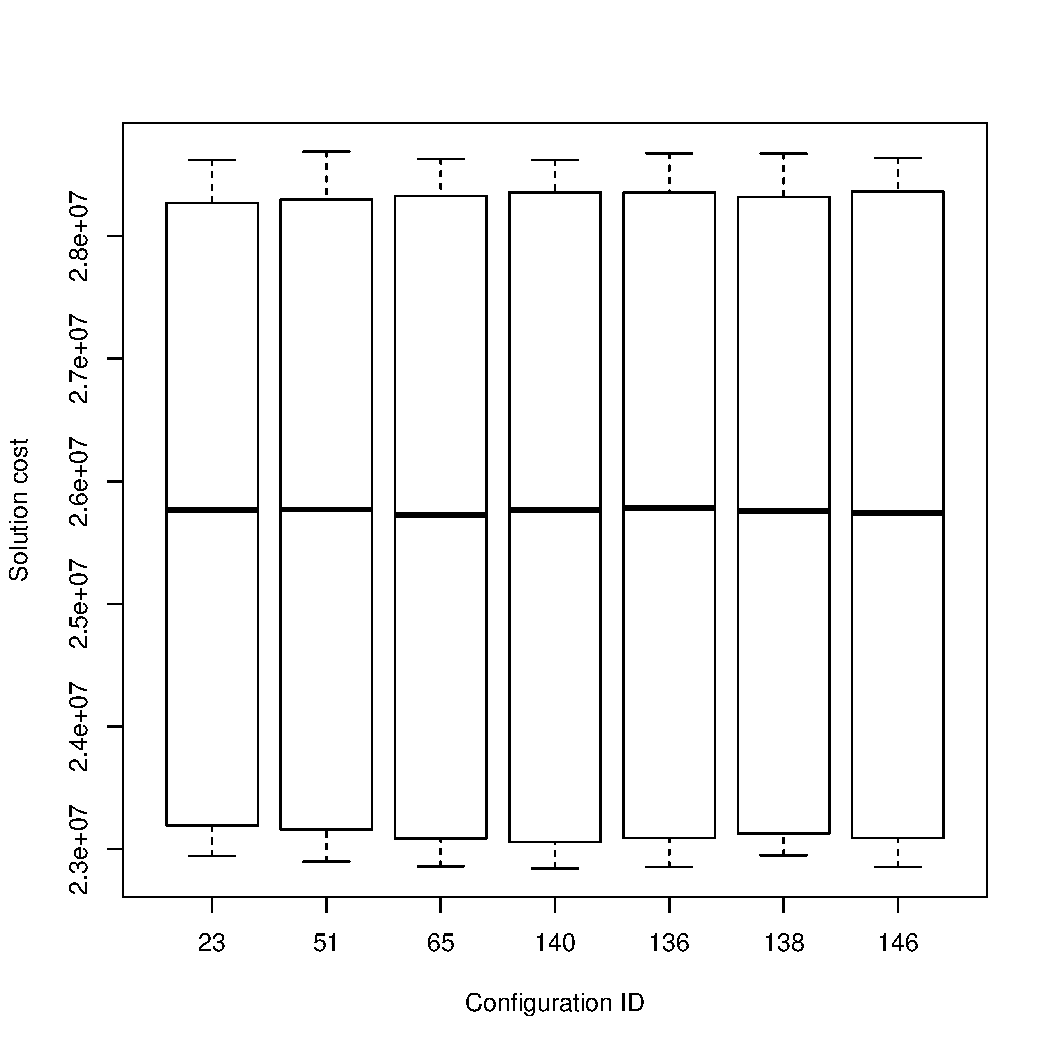
\includegraphics[width=0.75\textwidth]{figure/plot_test-1} 

}

\caption[Boxplot of the testing results of the best configurations]{Boxplot of the testing results of the best configurations.}\label{fig:plot_test}
\end{figure}


\end{knitrout}

%%FIXME: should we add something like this?
%The Kendall concordance coefficient (\code{W}) and the Spearman's rho can be
%applied over data that has the characteristics of the data obtained in the testing,
%that is a full matrix where all configurations are executed in all instances. \code{W}
%can show if the configurations tested have an homogeneous performance on the used instances
%set. If evidence of an heterogeneous scenario found we recommend to make some adjustments
%in the \irace options as described in \autoref{sec:}

%<<conc, prompt=TRUE, eval=TRUE, comment="">>=
%irace:::concordance(iraceResults$testing$experiments)
%@
%

During the tuning, \irace iteratively updates the sampling models of the
parameters to focus on the best regions of the parameter search space. The
frequency of the sampled configurations can provide insights on the parameter
search space. We provide a function for plotting the
frequency of the sampling of a set of configurations. For more information on this function, please see the \aR help, type in the
\aR console: \code{?parameterFrequency}. The following example
plots the frequency of the parameters sampled during one \irace run:

\begin{knitrout}
\definecolor{shadecolor}{rgb}{0.969, 0.969, 0.969}\color{fgcolor}\begin{kframe}
\begin{alltt}
\hlstd{> }\hlkwd{parameterFrequency}\hlstd{(iraceResults}\hlopt{$}\hlstd{allConfigurations, iraceResults}\hlopt{$}\hlstd{parameters)}
\end{alltt}
\begin{verbatim}
Plotting: algorithm 
Plotting: localsearch 
Plotting: alpha 
Plotting: beta 
Plotting: rho 
Plotting: ants 
Plotting: nnls 
Plotting: q0 
Plotting: dlb 
Plotting: rasrank 
Plotting: elitistants 
\end{verbatim}
\end{kframe}\begin{figure}[H]
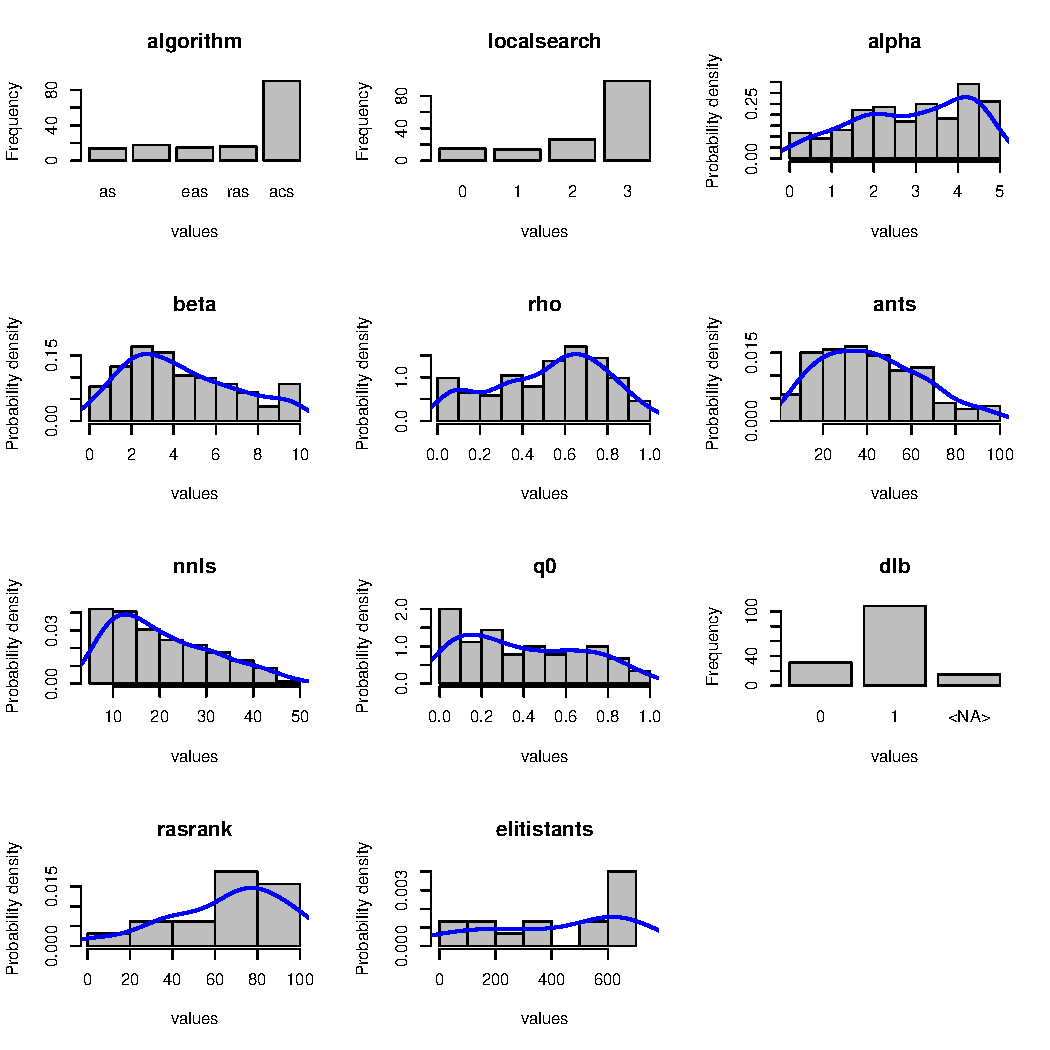
\includegraphics[width=\maxwidth]{figure/freq-1} \caption[Parameters sampling frequency]{Parameters sampling frequency.}\label{fig:freq}
\end{figure}


\end{knitrout}

By using parallel coordinates plots, it is possible to analyze how the parameters
interact with each other. For more information on this function, please see the \aR help, type
in the \aR console: (\code{?parallelCoordinatesPlot}).
 The following example shows how to create a parallel
coordinate plot of the configurations in the last two iterations of \irace.

\begin{knitrout}
\definecolor{shadecolor}{rgb}{0.969, 0.969, 0.969}\color{fgcolor}\begin{kframe}
\begin{alltt}
\hlcom{# Get last iteration number}
\hlstd{last} \hlkwb{<-} \hlkwd{length}\hlstd{(iraceResults}\hlopt{$}\hlstd{iterationElites)}
\hlcom{# Get configurations in the last two iterations}
\hlstd{conf} \hlkwb{<-} \hlkwd{getConfigurationByIteration}\hlstd{(}\hlkwc{iraceResults} \hlstd{= iraceResults,}
                                    \hlkwc{iterations} \hlstd{=} \hlkwd{c}\hlstd{(last} \hlopt{-} \hlnum{1}\hlstd{, last))}
\hlkwd{parallelCoordinatesPlot} \hlstd{(conf, iraceResults}\hlopt{$}\hlstd{parameters,}
                         \hlkwc{param_names} \hlstd{=} \hlkwd{c}\hlstd{(}\hlstr{"algorithm"}\hlstd{,} \hlstr{"alpha"}\hlstd{,}
                                         \hlstr{"beta"}\hlstd{,} \hlstr{"rho"}\hlstd{,} \hlstr{"q0"}\hlstd{),}
                         \hlkwc{hierarchy} \hlstd{=} \hlnum{FALSE}\hlstd{)}
\end{alltt}
\end{kframe}\begin{figure}[H]

{\centering 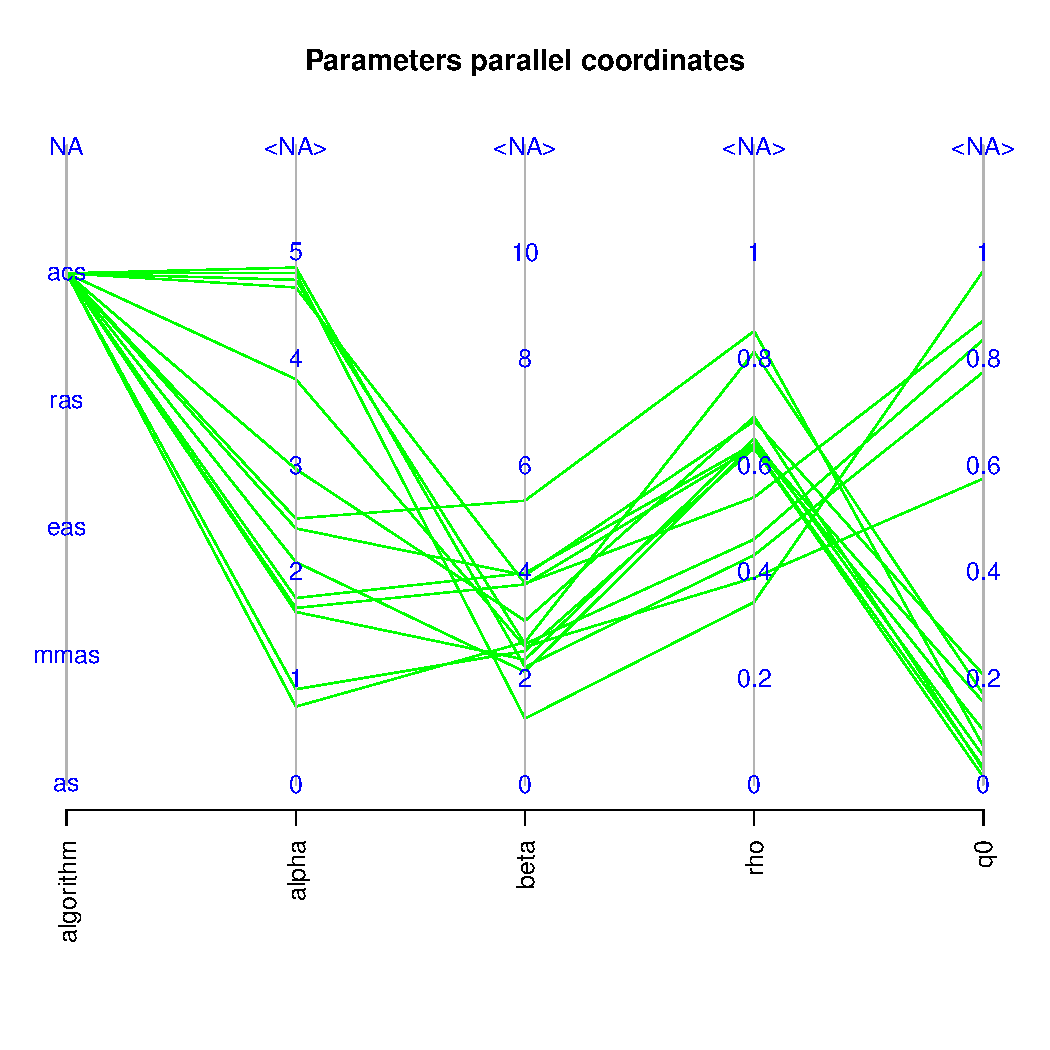
\includegraphics[width=0.75\textwidth]{figure/parcord-1} 

}

\caption[Parallel coordinate plots of the parameters of the configurations in the last two iterations of a run of \irace]{Parallel coordinate plots of the parameters of the configurations in the last two iterations of a run of \irace.}\label{fig:parcord}
\end{figure}


\end{knitrout}


\section{Advanced topics}

\subsection{Tuning budget}\label{sec:budget}

\Irace provides two options for setting the total tuning budget (\parameter{maxExperiments} and 
\parameter{maxTime}). Before setting the budget for the tuning, please consider the number of parameters that need to be tuned, available processing power 
and available time. The option \parameter{maxExperiments} 
limits the number of executions of \parameter{targetRunner} performed by \irace. The option \parameter{maxTime} limits the 
total time of the \parameter{targetRunner} executions. When this latter option is used, \parameter{targetRunner} 
must return the evaluation cost together with the execution time (\code{"cost time"}). 

\begin{xwarningbox}
When the goal is to minimize the computation time of an algorithm, and you wish to use \parameter{maxTime} as the tuning budget, \parameter{targetRunner} must return the time also as the evaluation cost, that is, return the time two times as \code{"time time"}.
\end{xwarningbox}

\begin{xwarningbox}
When using \parameter{targetEvaluator} and using \parameter{maxTime} as tuning budget, \parameter{targetRunner} just returns the time (\code{"time"}) and \parameter{targetEvaluator} returns the cost.
\end{xwarningbox}

When using \parameter{maxTime}, \irace estimates the execution time of each \parameter{targetRunner} execution 
before the configuration. The amount of budget used for the estimation is set with the option \parameter{budgetEstimation}
(default is $2\%$). The obtained estimation is adjusted after each iteration using the obtained results and it is used to estimate the number of experiments that can be executed. Internally, \irace uses the number of remaining experiments to 
adjust the number of configurations tested in each race. 

\subsection{Multi-objective tuning}\label{sec:multi objective}

Currently, \irace only optimizes one cost value at a time, which can be
solution cost, computation time or any other objective that is returned to
\irace by the \parameter{targetRunner}. If the target algorithm is
multi-objective, it will typically return not a single cost value, but a set of
objective vectors (typically, a Pareto front). For tuning such a target
algorithm with \irace, there are two alternatives. If the algorithm returns a
single vector of objective values, they can be aggregated into one single number
by using, for example, a weighted sum. Otherwise, if the target algorithm
returns a set of objective vectors, a unary quality metric (\eg~the
hypervolume) may be used to evaluate the quality of the set.\footnote{An implementation is publicly available at \url{http://lopez-ibanez.eu/hypervolume}~\cite{FonPaqLop06:hypervolume}}

% The first option is simple, it requires to devise a formula that can aggregate
% the objectives in a way that balances the importance of all of them. This might
% not be an easy task in some scenarios, and therefore using a more adequate
% indicator to evaluate the performance of a multi-objective optimizer, such as
% the hypervolume, is strongly advised.  

%For using the hypervolume as evaluation \irace needs to postpone the evaluation of the
%configurations in an instance until all the executions have been completed. Once
%the executions are finalized, the evaluation starts by obtaining reference points for 
%each objective from the configuration results. These points are used to define the 
%Pareto front and the hypervolume of each configuration
%is calculated and the tuning process continues normally.

The use of aggregation or quality metrics often requires normalizing the
different objectives. If normalization bounds are known a priori for each
instance, normalized values can be computed by \parameter{targetRunner}.
Otherwise, the bounds may be dynamically computed while running \irace, by
using \parameter{targetEvaluator}. In this case, \parameter{targetRunner} will
save the output of the algorithm, then the first call
to \parameter{targetEvaluator} will examine the output produced by all calls
to \parameter{targetRunner} for the same instance, update the normalization
bounds and return the normalized output. Subsequent calls
to \parameter{targetEvaluator} for the same instance will simply return the
normalized output.
%
A similar approach can be used to dynamically compute the reference points or
sets often required by unary quality metrics.

For more information about defining a \parameter{targetEvaluator}, see
\autoref{sec:evaluator}. Examples of tuning a multi-objective target algorithm
using the hypervolume can be found in the examples at
\IRACEHOME{/examples/hypervolume} and \IRACEHOME{/examples/moaco}.

\subsection{Tuning for minimizing computation time}

\Irace was developed primarily for tuning algorithms that report solution
cost. When using \irace for tuning algorithms that report computation time to
reach a target, the execution time of a configuration must be returned instead
of the cost by the \parameter{targetRunner}. Even though \irace can be used for
minimizing computation time, \irace may itself require more time to do so in
its current version than other methods, such as
\code{ParamILS}\footnote{\url{http://www.cs.ubc.ca/labs/beta/Projects/ParamILS/}}
or \code{SMAC}\footnote{\url{http://www.cs.ubc.ca/labs/beta/Projects/SMAC/}},
since it does not make use of techniques, such as ``adaptive capping'', that
avoid long runs of the target algorithm.

We are currently extending \irace with an adaptive capping mechanism.

\subsection{Heterogeneous scenarios}
\label{sec:het}

We classify a scenario as homogeneous when the target algorithm has a
consistent performance regarding the instances; roughly speaking, good
configurations tend to perform well and bad configurations tend to perform
poorly on all instances of the problem. By contrast, in heterogeneous
scenarios, the target algorithm has an inconsistent performance on different
instances, that is, some configurations perform well for a subset of the
instances, while they perform poorly for a different subset.

When facing a heterogeneous scenario, the first question should be whether the
objective of tuning is to find configurations that perform reasonably well over
all instances, even if they are not the best ones in any of them. If this is
not the case, then it would be better to partition instances into more similar
subsets and execute \irace separately on each subset. This will lead to a
portfolio of algorithm configurations, one for each subset, and algorithm
selection techniques can be used to select the best configuration from the
portfolio when facing a new instance.

If finding an overall good configuration for all the instances is the
objective, then we recommend that instances are randomly sampled
(option \parameter{sampleInstances}), unless one can provide the instances in a
particular order that does not bias the tuning towards any subset.  For
example, let's assume a heterogeneous scenario with two classes of instances.  If
training instances are not sampled and the first ten instances belong to only
one class, the tuning will be biased towards configurations that perform good
for those instances.  An optimal order would not ever present consecutively two
instances of the same type.

In addition, it may be useful to increase the number of instances executed
before doing a statistical test in order to see more instance classes before
discarding configurations. The option \parameter{elitistNewInstances} in elitist
\irace (option \parameter{elitist}) can be used to increase the number of new
instances executed in each iteration, \eg \code{--elitist-new-instances 5} (default
value is 1). For the non-elitist \irace, the option \parameter{firstTest} may be used for the same purpose, \eg \code{--first-test 10} (default value is 5).
\MANUEL{And both at the same time?}

While executing \irace, the homogeneity of the scenario can be observed by
examining the values of Spearman's rank correlation coefficient and Kendall's
concordance coefficient in the text output of \irace.  See \autoref{sec:output
  text} for more information.

\subsection{Choosing the statistical test}
\label{sec:stat test}

The statistical test used in \irace identifies statistically bad performing
configurations that can be discarded from the race in order to save
budget. Different statistical tests use different criteria to compare the
cost of the configurations, which has an effect on the tuning results.

\Irace provides two types of statistical tests
(option \parameter{testType}). Each test has different characteristics that are
beneficial for different goals:
%
\begin{itemize}
\item Friedman test (\code{F-test}): This test uses the ranking of the
  configurations to analyze the differences between their performance. This
  makes the test suitable for scenarios where the numerical results and their
  scale are not significant to assess the cost of the configurations.  For
  example, if the results for different instances have high numerical
  differences and evaluating the performance of the configurations using the
  mean could be deceiving.  We recommend to use the \code{F-test} (default)
  when tuning for solution cost and whenever the best performing algorithm
  should be among the best in as many instances as possible.
  
\item Student's t-test (\code{t-test}): This test uses the mean performance of
  the configurations to analyze the differences between the
  configurations. This makes the test suitable for scenarios where the
  differences between values obtained for different instances are relevant to
  assess good configurations.  We recommend using t-test, in particular, when
  the target algorithm is minimizing computation time and, in general, whenever
  the best configurations should obtain the best average solution cost.
\end{itemize}


The confidence level of the tests may be adjusted by using the
option \parameter{confidence}. Increasing the value of \parameter{confidence}
leads to a more strict statistical test.  Keep in mind that a stricter test
will require more budget to identify which configurations perform worse. A less
strict test discards configurations faster by requiring less evidence against
them and, therefore, it is more likely to discard good configurations.


\subsection{Complex parameters}

Some parameters may have complex dependencies. Ideally, parameters should be
defined in the way that is more likely to help the search performed by
\irace.  For example, when tuning a branch and bound algorithm, one may have the
following parameters:

\begin{itemize}
\item branching (\code{b}) that takes values in \code{\{0,1,2,3\}}, where 0 indicates no branching will be used
      and the rest are different types of branching.
\item stabilization (\code{s}) that takes values in \code{\{0,1,2,3,4,5,6,7,8,9,10\}}, of which for \code{b=0}
      only \code{\{0,1,2,3,4,5\}} are relevant.
\end{itemize}

In this case, it is not possible to describe the parameter space by defining
only two parameters for \irace. An extra parameter must be introduced as
follows:

\begin{center}
\begin{minipage}{0.8\linewidth}
\begin{CodeInput}
# name    label   type   range                    condition
b         "-b "   c      (0,1,2,3)
s1        "-s "   c      (0,1,2,3,4,5)            | b == "0"
s2        "-s "   c      (0,1,2,3,4,5,6,7,8,9,10) | b != "0"
  \end{CodeInput}
\end{minipage}
\end{center}

Parameters whose values depend on the value of other parameters may also
require using extra parameters or changing the parameters and processing them
in \parameter{targetRunner}. For example, given the following parameters:
%
\begin{itemize}
\item Population size (\code{p}) takes the integer values $[1,100]$.
\item Selection size (\code{s}) takes the same values but no more than the
  population size, that is $[1,$\code{p}$]$.
\end{itemize}

In this case, it is possible to describe the parameters \code{p} and \code{s}
using surrogate parameters for \irace that represent a ratio of the original
interval as follows:

\begin{center}
\begin{minipage}{0.8\linewidth}
\begin{CodeInput}
# name    label   type   range
p1        "-p "   r      (0.0,1.0)
s1        "-s "   r      (0.0,1.0)
\end{CodeInput}
\end{minipage}
\end{center}
%
and the values must be further processed in \parameter{targetRunner}. For
example, if the surrogate parameter \code{p1}  has value 0.5, mapping it to the
original interval of $[1,100]$, we obtain a value of $\text{\code{p}} =
51$. More than one value of the surrogate parameter (\eg 0.501 and 0.502)
result in the same final value. Parameter \code{s} has an interval that depends
on the final value of parameter \code{p}, if the surrogate parameter \code{s1} has value 0.3, it must be mapped to the interval $[1, 51]$, giving a value of $\text{\code{s}} = 16$.

The processing within \parameter{targetRunner} can also split and join
parameters. For example, assume the following parameters:

\begin{center}
\begin{minipage}{0.8\linewidth}
\begin{CodeInput}
# name    label   type   range
m         "-m "   i      (1,250)
e         "-e "   r      (0.0,2.0)
\end{CodeInput}
\end{minipage}
\end{center}

These parameters could be used to define a value
$\texttt{m}\cdot 10^\texttt{e}$ for another parameter
(\code{--strength}) not known by \irace. Then, \parameter{targetRunner} takes care of parsing
\code{-m} and \code{-e}, computing the strength value and passing the parameter
\code{--strength} together with its value to the target algorithm.

\subsection{Unreliable target algorithms}

There are some situations in which the target algorithm may fail to execute
correctly.  By default, \irace stops as soon as a call
to \parameter{targetRunner} or \parameter{targetEvaluator} fails, which helps to
detect bugs in the target algorithm.  Sometimes the failure cannot be fixed
because it is due to system problems, network issues, memory limits, bugs for
which no fix is available, or fixing them is impossible because there is no
access to the source code.

In those cases, if the failure is caused by random errors or transient system
problems, one may wish to ignore the error and try again the same call in the
hope that it succeeds. The option \parameter{targetRunnerRetries} indicates the
number of times a \parameter{targetRunner} execution is repeated if it
fails. Use this option only if you know additional repetitions could be
successful.

If the target algorithm consistently fails for a particular set of
configurations, these configurations may be declared as forbidden
(\parameter{forbiddenFile}) so that \irace avoids them.  On the other hand, if
the configurations that cause the problem are unknown,
the \parameter{targetRunner} script should detect the failure and return a
penalty cost (a very large cost value) so that \irace discards the failing
configuration as soon as possible.  The penalty must be set according to the
range of the cost measure and the goals of the tuning. For example, a
configuration that crashes on a particular instance, \eg by running out of
memory, might still be considered acceptable if it gives very good results on
other instances.


\section{List of command-line and scenario options} \label{sec:irace options}

Most \irace options can be specified in the command line using a flag or in the
\irace scenario file using the option name (or setting their value in the
\code{scenario} list passed to the various \aR functions exported by the
package). This section describes the various \irace options that can be
specified by the user in this way.

\subsection{General options}
\begin{description}
\defparameter[s]{scenarioFile}{scenario}{./scenario.txt} %
  File that contains the scenario setup and other irace options. All options listed in this section
  can be included in this file. See \IRACEHOME{/templates/} for an example.

\defparameter{debugLevel}{debug-level}{0} %
  Level of information to display in the text output of \irace. A value of 0 silences all debug messages.
  Higher values provide more verbose debug messages. To see details about the text output of \irace, see
  \autoref{sec:output text}.

\defparameter{seed}{seed}{NA} %
  Seed to initiallize the random number generator. The seed must be a positive integer. If the seed is
  \code{NA}, a random seed will be generated.

\defparameter{execDir}{exec-dir}{./} %
  Directory where the target algorithm executions will be performed. The default execution directory is the current directory.
  \begin{xwarningbox}
    The execution directory must exist
    before executing \irace, it will not be created automatically.
 \end{xwarningbox}

\defparameter[l]{logFile}{log-file}{./irace.Rdata} %
  File to save tuning results as an \aR dataset. The provided path must be either an absolute path
  or relative to \parameter{execDir}. See \autoref{sec:output r} for details on the format of the
  R dataset.

\defparameter{repairConfiguration}{}{NULL} %
User-defined \aR function that takes a configuration generated by irace and repairs it. See \autoref{sec:repairconf} for details.

\end{description}

\subsection{Elitist \irace}
\begin{description}
\defparameter{elitist}{elitist}{1} %
  Enable/disable elitist \irace.

  In the \textbf{elitist} version of \code{irace}~\citep{LopDubPerStuBir2016irace}, elite configurations are not
  discarded from the race until non-elite configurations have been executed on
  the same instances as the elite configurations.

  Each race begins by evaluating all configurations on a number of new
  instances. This number is defined by the option \parameter{elitistNewInstances}.
  After the new instances have been evaluated, configurations are evaluated on
  instances seen in the previous race.  Elite configurations already have
  results for most of these previous instances and, therefore, do not need to
  be re-evaluated. Finally, after configurations have been evaluated on all
  these instances, the race continues by evaluating additional new instances.

  The statistical tests can be performed at any moment during the race
  according to the setting of the options \parameter{firstTest}
  and \parameter{eachTest}. The elitist rule forbids discarding elite
  configurations, even if the show poor performance, until the last of the
  previous instances is seen in the race.

  The \textbf{non-elitist} version of \irace can discard elite configurations
  at any point of the race, instances are not re-used from one race to the
  next, and new instances are sampled for each race.
  %% MANUEL: This does not make sense to me. Isn't this the same for elitist?
  % are always executed unless the
  % \parameter{deterministic} option is active and all instances have already been used.

  \defparameter{elitistNewInstances}{elitist-new-instances}{1} %
  Number of new instances added to each race before evaluating instances from
  previous races (only for elitist \irace).
  \begin{xwarningbox}
  If \parameter{deterministic} is \code{TRUE} then the number of \parameter{elitistNewInstances} will be reduced or
  set to \code{0} once all instances have been evaluated.
  \end{xwarningbox}

  \defparameter{elitistLimit}{elitist-limit}{2} %

  Maximum number of statistical tests performed without successful elimination
  after all instances from the previous race have been evaluated. If the limit
  is reached, the current race is stopped. Only valid for elitist \irace. Use 0
  to disable the limit.
\end{description}


\subsection{Internal \irace options}
\begin{description}
\defparameter{sampleInstances}{sample-instances}{1} %
  Enable/disable the sampling of the training instances. If the option \parameter{sampleInstances} is disabled,
  the instances are used in the order provided in the \parameter{trainInstancesFile} or in the order they
  are read from the \parameter{trainInstancesDir} when\parameter{trainInstancesFile} is not provided. For more
  information about training instances see \autoref{sec:training}.

  \defparameter{nbIterations}{iterations}{0} %
  Minimum number of iterations to be executed. Each iteration involves the
  generation of new configurations and the use of racing to select the best
  configurations. By default (with 0), \irace calculates the minimum number of
  iterations as $\Niter = \lfloor 2 + \log_{2}\Nparam \rfloor$, where $\Nparam$
  is the number of non-fixed parameters to be tuned.
  %
  We recommend to use the default value.

\defparameter{nbExperimentsPerIteration}{experiments-per-iteration} {0} %
  Number of experiments to execute per iteration. By default (when equal to 0), this value changes for each iteration and depends on the iteration index and the remaining budget. Further details are provided in the \irace paper~\citep{LopDubPerStuBir2016irace}.
  % \irace calculates the number of experiments per iteration based as follows:
  % \begin{equation}
  %   \Budgetj = \dfrac{(\Budget - \Bused)}{ (\Niter -\iter + 1)}
  % \end{equation}
  % %
  % where $\Budgetj$ is the budget for iteration $j$, $\Budget$ is the total
  % tuning budget (\parameter{maxExperiments}), $\Bused$ is the used budget and $\Niter$ is maximum between the planned number of
  %  iterations (\parameter{nbIterations}) and the current iteration ($j$). 
  %  
  We recommend to use the default value.

\defparameter{nbConfigurations}{num-configurations}{0} %
  The number of configurations that will be raced at each iteration. By default
  (when equal to 0), this value changes for each iteration and depends
  on \parameter{nbExperimentsPerIteration}, the iteration index
  and \parameter{mu}. The precise details are given in the \irace
  paper~\citep{LopDubPerStuBir2016irace}.
  % \irace
%   calculates the number of configurations per iteration as follows:\begin{equation}
%   \Ncand[\iter] = \left\lfloor \frac{\Budgetj} { (\mu + \min(5,\iter))}\right\rfloor
%   \end{equation}
% %
%   where $\Ncand[\iter]$ is the
%   number of configurations that will be used in iteration $j$, $\Budgetj$ is the budget for iteration $j$ and $\mu$ is the 
%   option \parameter{mu}.
  We recommend to use the default value.
  
  \defparameter{mu}{mu}{5} %
  This value is used to determine the number of configurations to be sampled
  and evaluated at each iteration. The number of configurations will be
  calculated such that there is enough budget in each race to evaluate all
  configurations on at least $\mu + \min(5,j)$ training instances, where $j$ is
  the index of the current iteration. The value of $\mu$ will be adjusted to
  never be lower than the value of \parameter{firstTest}. We recommend to use
  the default value and, if needed, adjust \parameter{firstTest}
  and \parameter{eachTest}, instead.


\defparameter{minNbSurvival}{min-survival}{0} %
  The minimum number of configurations needed to continue the execution of a
  race. If the number of configurations alive in the race is not larger than
  this value, the current iteration will stop and a new iteration will start, even if there is budget left to continue the current race.
  By default (when equal to 0), the value is calculated
  automatically as $\lfloor 2 + \log_{2}\Nparam \rfloor$, where $\Nparam$
  is the number of non-fixed parameters to be tuned.

\defparameter{softRestart}{soft-restart}{1} %
  Enable/disable the soft-restart strategy that avoids premature convergence of the probabilistic model.
  When a sampled configuration is \emph{similar} to its parent configuration, the probabilistic model
  of these configurations is soft restarted. The soft-restart mechanism is explained in the \irace paper~\citep{LopDubPerStuBir2016irace}. The similarity of categorical and ordinal parameters is given
  by the hamming distance, and the option \parameter{softRestartThreshold} defines the similarity of numerical parameters. 


\defparameter{softRestartThreshold}{soft-restart-threshold}{NA} %
  Soft restart threshold value for numerical parameters. If \code{NA}, it is computed as $10^{-digits}$, where
  \parameter{digits} corresponds to the \irace option explained in this section.

\end{description}

\subsection{Target algorithm parameters}
\begin{description}

\defparameter[p]{parameterFile}{param-file}{./parameters.txt} %
  File that contains the description of the parameters of the target algorithm. See \autoref{sec:target parameters}.

\defparameter{digits}{digits}{4} %
  Maximum number of decimal places that are significant for numerical (real) parameters.

\defparameter{forbiddenFile}{forbidden-file}{} %
  File containing a list of logical expressions that cannot be true for any evaluated configuration. If
  empty or \code{NULL}, no forbidden configurations are considered. See \autoref{sec:forbidden} for more information.

\end{description}

\subsection{Target algorithm execution}
\begin{description}

\defparameter{targetRunner}{target-runner}{./target-runner} %
  This option defines a script or an \aR function that evaluates a configuration of the target algorithm on a particular instance. See \autoref{sec:runner} for details.

\defparameter{targetRunnerRetries}{target-runner-retries}{0} %
  Number of times to retry a call to \parameter{targetRunner} if the call failed.

\defparameter{targetRunnerData}{}{NULL} %
Optional data passed to \parameter{targetRunner}. This is ignored by the default \parameter{targetRunner} function, but it may be used by custom \parameter{targetRunner} functions to pass persistent data around.

\defparameter{targetRunnerParallel}{}{NULL} %
 Optional \aR function to provide custom parallelization of \parameter{targetRunner}. See \autoref{sec:parallel}
 for more information.

\defparameter{targetEvaluator}{target-evaluator}{""} %
  Optional script or \aR function that returns a numerical value for an experiment after all configurations have been executed on a given instance using \parameter{targetRunner}. See \autoref{sec:evaluator} for details.

\defparameter{deterministic}{deterministic}{0} %
  Enable/disable deterministic target algorithm mode. If the target algorithm is deterministic, configurations will be evaluated only once per instance. See \autoref{sec:training} for more information.
  \begin{xwarningbox}
  If the number of instances provided is less than the value
  specified for the option \parameter{firstTest}, no statistical test will be performed.
  \end{xwarningbox}

\defparameter{parallel}{parallel}{0} %
  Number of calls of the \parameter{targetRunner} to execute in parallel. A value of 0 means no parallelization. For more information
  on parallelization, see \autoref{sec:parallel}.

\defparameter{loadBalancing}{load-balancing}{1} %
  Enable/disable load-balancing when executing experiments in parallel. Load-balancing makes better use of computing
  resources, but increases communication overhead. If this overhead is large, disabling load-balancing may be faster.
  See \autoref{sec:parallel}.

\defparameter{mpi}{mpi}{0} %
  Enable/disable use of \pkg{Rmpi} to execute the \parameter{targetRunner} in parallel using MPI protocol. When \parameter{mpi} is
  enabled, the option \parameter{parallel} is the number of slave nodes. See \autoref{sec:parallel}.

\defparameter{batchmode}{batchmode}{0} %
  Specify how irace waits for jobs to finish when \parameter{targetRunner} submits jobs to
  a batch cluster: sge, pbs, torque or slurm (\parameter{targetRunner} must
  submit jobs to the cluster using. for example, \code{qsub}). See
  \autoref{sec:parallel}.

 
\end{description}

\subsection{Initial configurations}
\begin{description}
\defparameter{configurationsFile}{configurations-file}{} %
  File containing a list of initial configurations. If empty or \code{NULL}, \irace will not use initial
  configurations. See \autoref{sec:initial}.

  \begin{xwarningbox}
    The provided configurations must not violate the constraints described in \parameter{parameterFile}
    and \parameter{forbiddenFile}.
  \end{xwarningbox}
\end{description}


\subsection{Training instances}
\begin{description}
\defparameter{trainInstancesDir}{train-instances-dir}{./Instances} %
  Directory where tuning instances are located; either absolute path or relative to current directory. See \autoref{sec:training}.

\defparameter{trainInstancesFile}{train-instances-file}{} %
  File containing a list of instances and optionally additional parameters for them. See \autoref{sec:training}.
  \begin{xwarningbox}
  If \parameter{trainInstancesDir} is specified, the path contained in \parameter{trainInstancesFile} must be relative to the directory. When using an absolute path or for defining instances that are not files, set \code{trainInstancesDir=""}.
\end{xwarningbox}
\end{description}

\subsection{Tuning budget}

\begin{description}
\defparameter{maxExperiments}{max-experiments}{0}
  The maximum number of runs (invocations of \parameter{targetRunner}) that will be performed. It determines the maximum budget
  of experiments for the tuning. See \autoref{sec:budget}.
  \defparameter{maxTime}{max-time}{0}
  The maximum total time in seconds for the runs of \parameter{targetRunner} that will be 
  performed. The mean execution time  of each run is estimated in order to calculate the maximum number of experiments (see option \parameter{budgetEstimation}). 
  When \parameter{maxTime} is positive, then \parameter{targetRunner} \textbf{must} return the execution time as its second output. See \autoref{sec:budget}.
  
\defparameter{budgetEstimation}{budget-estimation}{0.02}
  The percentage of the budget used for estimating the mean execution time. Only used when \parameter{maxTime} $> 0$. See \autoref{sec:budget}.

\end{description}

\subsection{Statistical test}
\begin{description}
\defparameter{testType}{test-type}{F-test} %
  Specifies the statistical test type:
  \begin{itemize}
    \item[] \code{F-test} (Friedman test)
    \item[] \code{t-test} (pairwise t-tests with no correction)
    \item[] \code{t-test-bonferroni} (t-test with Bonferroni's correction for multiple comparisons)
    \item[] \code{t-test-holm} (t-test with Holm's correction for multiple comparisons).
  \end{itemize}
  We recommend to not use corrections for multiple comparisons because the test typically becomes too strict and the search stagnates. 
  See \autoref{sec:stat test} for details about choosing the statistical test most appropriate for your scenario.

\defparameter{firstTest}{first-test}{5} %
  Specifies how many instances are evaluated before the first elimination test.
  \begin{xwarningbox}%
   The value of \parameter{firstTest} must be a multiple of \parameter{eachTest}.
  \end{xwarningbox}

\defparameter{eachTest}{each-test}{1} %
  Specifies how many instances are evaluated between elimination tests.

\defparameter{confidence}{confidence}{0.95}
  Confidence level for the elimination test.

\end{description}

\subsection{Recovery}
\label{sec:recovery}

\begin{description}
\defparameter{recoveryFile}{recovery-file}{""}  %
  Previously saved \irace log file that should be used to recover the execution of \irace;
  either absolute path or relative to the current directory. If empty or \code{NULL}, recovery is not performed.
  For more details about recovery, see \autoref{sec:recovery}.

\end{description}

\subsection{Testing}
\begin{description}
\defparameter{testNbElites}{test-num-elites}{1} %
  Number of elite configurations returned by irace that will be tested if test instances are provided. For more information
  about the testing, see \autoref{sec:testing}.

\defparameter{testIterationElites}{test-iteration-elites}{0} %
  Enable/disable testing the elite configurations found at each iteration.

\defparameter{testInstancesDir}{test-instance-dir}{} %
  Directory where testing instances are located, either absolute or relative to the current directory.

\defparameter{testInstancesFile}{test-instance-file}{} %
  File containing a list of test instances and, optionally, additional parameters for them.
  
\defparameter{-{}-only-test}{}{} %
Run the configurations provided in the file argument on the test instances. See \autoref{sec:testing}.
  
\end{description}

\section{FAQ}

\subsection{Is \irace minimizing or maximizing the output of my algorithm?}

By default, \irace considers that the value returned by \parameter{targetRunner} (or by
\parameter{targetEvaluator}, if used) should be \underline{\textbf{minimized}}. In case of a maximization
problem, one can simply multiply the value by -1 before returning it to
irace. This is done, for example, when maximizing the hypervolume (see the last
lines in \IRACEHOME{/examples/hypervolume/target-evaluator}).


\subsection{Is it possible to configure a MATLAB algorithm with \irace?}

Definitely. There are two main ways to achieve this:
\begin{enumerate}
\item{ Edit the \parameter{targetRunner} script to call MATLAB in a non-interactive
    way. See the MATLAB documentation, or the following links.\footnote{\url{http://stackoverflow.com/questions/1518072/suppress-start-message-of-matlab}\\ \url{http://stackoverflow.com/questions/4611195/how-to-call-matlab-from-command-line-and-print-to-stdout-before-exiting}} %
    You would need to pass the parameter received by \parameter{targetRunner} to your MATLAB script: \url{http://www.mathworks.nl/support/solutions/en/data/1-1BS5S/?solution=1-1BS5S}. There is a minimal example in:
    \begin{center}
      \IRACEHOME{/examples/matlab/}.
    \end{center}
  }
\item{ Call MATLAB code directly from \aR using the
    \pkg{R.matlab} package (\url{https://cran.r-project.org/package=R.matlab}). This
    is a better option if you are experienced in \aR. Define \parameter{targetRunner} as
    an \aR function instead of a path to a script. The function should
    call your MATLAB code with appropriate parameters.
  }
\end{enumerate}

\subsection{My program works perfectly on its own, but not when running under \irace. Is irace broken?}\label{faq:valgrind}

Every time this was reported, it was a difficult-to-reproduce bug in
the program, not in \irace.  We recommend that in \parameter{targetRunner}, you use
\code{valgrind} to run your program. That is, if your program is called like:
% 
\begin{lstlisting}[style=BashInputStyle]
    $EXE ${FIXED_PARAMS} -i $INSTANCE ${CONFIG_PARAMS} \
     1> ${STDOUT} 2> ${STDERR}
\end{lstlisting}
%
then replace that line with:
% 
\begin{lstlisting}[style=BashInputStyle]
   valgrind --error-exitcode=1 $EXE ${FIXED_PARAMS} \
    -i $INSTANCE ${CONFIG_PARAMS} 1> ${STDOUT} 2> ${STDERR}
\end{lstlisting}

If there are bugs in your program, they will appear in \code{${STDERR}}, thus do not delete those files.


\subsection{My program may be buggy and run into an infinite loop. Is it possible to set a maximum timeout?}\label{faq:timeout}

We are not aware of any way to achieve this using \aR. However, in
GNU/Linux, it is easy to implement by using the \code{timeout} command in
\code{targetRunner} when invoking your program.

\subsection{When using the mpi option, \irace is aborted with an error message indicating that a
  function is not defined. How to fix this?}\label{sec:mpi-error}

\pkg{Rmpi} does not work the same way when called from within a package and when called from a script or 
interactively. When \irace creates the slave nodes, the slaves will load a copy of \irace automatically. 
If the slave nodes are on different machines, they must have \irace installed. If \irace is not installed
system-wide, \aR needs to be able to find \irace on the slave nodes. This is usually done by setting \code{R\_LIBS}, 
\code{.libPaths()} or by loading \irace using \code{library()} or \code{require()} with the argument ``\code{lib.loc}''. 
The settings on the master are not applied to the slave nodes automatically, thus the slave 
nodes may need their own settings. After spawning the slaves, it is too late to modify 
those settings, thus modifying the shell variable \code{R\_LIBS} seems the only valid 
way to tell the slaves where to find \irace.

If the path is set correctly and the problem persists, please check these instructions:
% 
\begin{enumerate}[leftmargin=*,widest=3]
\item Test that \irace and \pkg{Rmpi} work. Run \irace on a single machine (submit node), without calling \code{qsub}, \code{mpirun} or a 
  similar wrapper around \irace or \aR.
\item Test loading \irace on the slave nodes. However,
  jobs submitted by \code{qsub}/\code{mpirun} may load \aR packages using a different mechanism from the way it happens if you log directly into the node (e.g., with \code{ssh}). Thus, you need to write a little \aR program such as:
\begin{knitrout}
\definecolor{shadecolor}{rgb}{0.969, 0.969, 0.969}\color{fgcolor}\begin{kframe}
\begin{alltt}
\hlkwd{library}\hlstd{(Rmpi)}
\hlkwd{mpi.spawn.Rslaves}\hlstd{(}\hlkwc{nslaves} \hlstd{=} \hlnum{10}\hlstd{)}
\hlstd{x} \hlkwb{<-} \hlkwd{mpi.applyLB}\hlstd{(}\hlnum{1}\hlopt{:}\hlnum{10}\hlstd{,} \hlkwa{function}\hlstd{(}\hlkwc{x}\hlstd{) \{}
  \hlkwd{library}\hlstd{(irace)}
  \hlkwd{return}\hlstd{(}\hlkwd{path.package}\hlstd{(}\hlstr{"irace"}\hlstd{)) \})}
       \hlkwd{print}\hlstd{(x)}
\end{alltt}
\end{kframe}
\end{knitrout}
      Submit this program to the cluster (using \code{qsub}/\code{mpirun}) like you would submit \irace.
      
      \item In the script \code{bin/parallel-irace-mpi}, the function \code{irace\_main()} creates an MPI job for our cluster. 
      You may need to speak with the admin of your cluster and ask them how to best submit a job for MPI. There may be 
      some particular settings that you need. \pkg{Rmpi} normally creates  log files; but \irace suppresses those files unless $\texttt{debugLevel} > 0$.
     \end{enumerate}
     
     Please contact us (\autoref{sec:contact}) if you have further problems.

\subsection[Error: 4 arguments passed to {.Internal(nchar)} which requires 3]{Error: 4 arguments passed to \code{.Internal(nchar)} which requires 3}

This is a bug in \aR 3.2.0 on Windows. The solution is to update your version of
\aR.
     
%FIXME: complete this section
%\section{Known problems}

\section{Resources and contact information} \label{sec:contact}

More information about the package can be found on the \irace webpage:
\begin{center} \url{http://iridia.ulb.ac.be/irace/} \end{center}

For questions and suggestions please contact the development team through 
the \irace package Google group:
\begin{center}
  \url{https://groups.google.com/d/forum/irace-package}
\end{center} 
or by sending an email to:
\begin{center}
  \href{mailto:irace-package@googlegroups.com}{irace-package@googlegroups.com}
\end{center}

%% MANUEL: I think we should use just one channel. If the Google group is the winner, that should be it.
%the mailing list:
%% LESLIE I agree.
%\begin{center} \href{mailto:irace@iridia.ulb.ac.be}{irace@iridia.ulb.ac.be} \end{center}


\section{Acknowledgements}

We would like to thank all the people that directly or indirectly have
collaborated in the development and improvement of \irace:
%
\newlist{acklist}{itemize*}{1}
\setlist[acklist]{label={}, before=\unskip{}, afterlabel=\unskip{ }, itemjoin={{,}}, itemjoin*={, and }, after={{.}}}
\begin{acklist}
\item Prasanna Balaprakash
\item Zhi (Eric) Yuan
\item Franco Mascia
\item Alberto Franzin
\item Anthony Antoun
\item Esteban Diaz Leiva %MATLAB example
\item Federico Caselli % bug reports with fixes
\item Pablo Valledor Pellicer % testing of --parallel under Windows
\end{acklist}


\bibliographystyle{abbrvnat}
\ifthenelse {\boolean{Release}}{%
\bibliography{irace-package}%
}{%
\bibliography{optbib/abbrev,optbib/journals,optbib/authors,optbib/biblio,optbib/crossref}%
}

\newpage

\begin{appendices}

\section{Installing R} \label{sec:installation}

This section gives a quick \aR installation guide that will work in
most cases. The official instructions are available at
\url{https://cran.r-project.org/doc/manuals/r-release/R-admin.html}

\subsection{GNU/Linux}
You should install \aR from your package manager. On a Debian/Ubuntu system
it will be something like:
\begin{lstlisting}[style=BashInputStyle]
sudo apt-get install r-base
\end{lstlisting}

Once \aR is installed, you can launch \aR from the Terminal and from the \aR prompt
install the \irace package (see \autoref{sec:irace install}).


\subsection{OS X}

You can install \aR directly from a CRAN mirror.\footnote{\url{https://cran.r-project.org/bin/macosx/}} %
Alternatively, if you use
homebrew, you can just brew the \aR formula from the science tap (unfortunately
it does not come already bottled so you need to have Xcode\footnote{Xcode download
webpage: \url{https://developer.apple.com/xcode/download/}} installed to compile it):
%<<R_OS_install,engine='bash',eval=FALSE>>=
\begin{lstlisting}[style=BashInputStyle]
brew tap homebrew/science
brew install r
\end{lstlisting}
%@

Once \aR is installed, you can launch \aR from the Terminal (or from your Applications),
and from the \aR prompt install the \irace package (see \autoref{sec:irace install}).

\subsection{Windows}

You can install \aR from a CRAN mirror.\footnote{\url{https://cran.r-project.org/bin/windows/}} %
We recommend that you
install \aR on a filesystem path without spaces, special characters or long
names, such as \path{C:\R}. Once \aR is installed, you can launch the \aR
console and install the \irace package from it (see \autoref{sec:irace
  install}).


\section{targetRunner troubleshooting checklist} \label{sec:check list}

If the \parameter{targetRunner} script fails to return the output expected by
\irace, it can be sometimes difficult to diagnose where the problem lies. The
more descriptive errors provided by your script, the easier it will be to debug
it. If \parameter{targetRunner} enters an infinite loop, irace will wait
indefinitely (see FAQ in \autoref{faq:timeout}).  If you are using temporary
files to redirect the output of your algorithm, check that these files are
properly created. We recommend to follow the structure of the example file
(\code{target-runner}) provided in \IRACEHOME{/templates}. The following
error examples are based on a file with those characteristics.

In case of failure of \parameter{targetRunner}, \irace will print an error on
its output describing which execution of \parameter{targetRunner} was not
successful.
%
Follow this checklist to detect where the problem is:

\begin{enumerate}[leftmargin=*,widest=9]

\item Make sure that your \code{targetRunner} script or program is at the specified location. If you see this error:
\begin{CodeInput}
Error: == irace == target runner '~/tuning/target-runner' does not exist
\end{CodeInput}
%
it means that \irace cannot find the \code{target-runner} file. Check that the file is at
the path specified by the error.

\item Make sure that your \code{targetRunner} script is an executable file and the user running \irace has permission to execute it. The following errors:
%
\begin{CodeInput}
Error: == irace == target runner '~/tuning/target-runner' is a directory,
not a file
\end{CodeInput}
or
\begin{CodeInput}
Error: == irace == target runner '~/tuning/target-runner' is not executable
\end{CodeInput}
%
mean that your \code{targetRunner} is not an executable file. In the first
case, the script is a folder and therefore there must be a problem with the
name of the script. In the second case, you must make the file executable,
which in GNU/Linux can be done by:
%
\begin{lstlisting}[style=BashInputStyle]
chmod +x ~/tuning/target-runner
\end{lstlisting}

\item If your \code{targetRunner} script calls another program, make sure it is at  the location described in the script
(variable \code{EXE} in the examples and templates). A typical output for such an error is:
%
\begin{CodeInput}
Error: == irace == running command ''~/tuning/target-runner' 1 8 676651103 
~/tuning/Instances/1000-16.tsp --ras --localsearch 2 --alpha 4.03 --beta 1.89
--rho  0.02 --ants 37 --nnls 48 --dlb 0 --rasranks 15 2>\&1' had status 1  
== irace == The call to target.runner.default was:
~/tuning/target-runner 1 8 676651103 ~/tuning/Instances/1000-16.tsp --ras 
--localsearch 2 --alpha 4.03 --beta 1.89 --rho  0.02 --ants 37 --nnls 48 
--dlb 0 --rasranks 15 
== irace == The output was:
Tue May  3 19:00:37 UTC 2016: error: ~/bin/acotsp: not found or not executable
(pwd: ~/tuning/acotsp-arena)
\end{CodeInput}
%
You may test your script by copying the command line shown in the error and
executing \code{target-runner} directly on the execution directory (\parameter{execDir}). In this case, the command line is:
%
\begin{lstlisting}[style=BashInputStyle]
~/tuning/target-runner 1 8 676651103 ~/tuning/Instances/1000-16.tsp  --ras \
 --localsearch 2 --alpha 4.03 --beta 1.89 --rho  0.02 --ants 37 --nnls 48 \
 --dlb 0 --rasranks 15
\end{lstlisting}

This executes the \code{targetRunner} script as \irace does. The output of this script must be only one number. 

\item Check that your \code{targetRunner} script is actually returning one
  number as output. If you see an error as the following, this is your problem:
% 
\begin{CodeInput}
Error: == irace == The output of '~/tuning/target-runner 
1 25 365157769 ~/tuning/Instances/1000-31.tsp --ras 
--localsearch 1 --alpha 0.26  --beta 6.95 --rho  0.69 
--ants 56 --nnls 10 --dlb 0 --rasranks 7' is not numeric! 
== irace == The output was:
Solution: 24479793
\end{CodeInput}
%
For testing your script, copy the command-line of \code{target-runner} and execute it directly on the execution directory (\parameter{execDir}):
%
\begin{lstlisting}[style=BashInputStyle]
~/tuning/target-runner 1 25 365157769 ~/tuning/Instances/1000-31.tsp  --ras \
 --localsearch 1 --alpha 0.26 --beta 6.95 --rho  0.69 --ants 56 \
 --nnls 10 --dlb 0 --rasranks 7
\end{lstlisting}

This  executes the \code{targetRunner} script as \irace does. The output of this
script must be only one number. In this example, the output of the script is
``\code{Solution: 24479793}'', which is not a number. The code that \code{targetRunner} uses to parse the output of the algorithm must be checked.

\item Check that your \code{targetRunner} script is creating the output files
  for your algorithm.  If you see an error as:
%
\begin{CodeInput}
== irace == The output was: Tue May  3 19:41:40 UTC 2016: 
error: c1-9.stdout: No such file or directory
\end{CodeInput}
The output file of the execution of your algorithm has not been
created (check permissions) or has been deleted before the result can be read.


\item Other errors can produce the following output:
%
\begin{CodeInput}
== irace == The output was: Tue May  3 19:49:06 UTC 2016: 
error: c1-23.stdout: Output is not a number
\end{CodeInput}
%
This might be because your \code{targetRunner} script is not executing your
algorithm correctly. To further investigate this issue, comment out the line
that eliminates the temporary files that saves the output of your
algorithm. Similar to this one
%
\begin{lstlisting}[style=BashInputStyle]
rm -f "${STDOUT}" "${STDERR}"
\end{lstlisting}
%
Execute directly the \code{targetRunner} command-line that is provided in the
error message, look in your execution directory for the files that are
created. Check the \code{.stderr} file for errors and the \code{.stdout} file
to see the output that your algorithm produces.

\item It is possible that transient bugs in the target algorithm are only
  visible when running within \irace, and \code{targetRunner} appears to work
  fine when executed directly in the command-line outside \irace (See FAQ in \autoref{faq:valgrind}).
  %
  We recommend that in \parameter{targetRunner}, you use
     \code{valgrind} to run your program. That is, if your program is called like:
     % 
\begin{lstlisting}[style=BashInputStyle]
    $EXE ${FIXED_PARAMS} -i $INSTANCE ${CONFIG_PARAMS} \
     1> ${STDOUT} 2> ${STDERR}
\end{lstlisting}
%
     then replace that line with:
%
\begin{lstlisting}[style=BashInputStyle]
   valgrind --error-exitcode=1 $EXE ${FIXED_PARAMS} \
    -i $INSTANCE ${CONFIG_PARAMS} 1> ${STDOUT} 2> ${STDERR}
\end{lstlisting}
     
     If there are bugs in your program, they will appear in \code{${STDERR}}, thus do not delete those files.


\item If your \code{targetRunner} script works when running irace with \code{parallel=1} but it fails when using higher number of cores, this may be due to any number of reasons:
  \begin{itemize}
  \item If you submit jobs through a queuing system, the running environment
    when using the queuing system may not be the same as when you launch \irace
    yourself. The queuing system may also send the job to different machines
    depending on the number of CPUs requested. One way to test this is to
    submit the failing execution of \code{targetRunner} to the queuing system,
    and specifically to any problematic machine.
    
  \item When using MPI, some calls to \code{targetRunner} may run on different
    computers than the one running the master \irace process. See FAQ in
    \autoref{sec:mpi-error}.
    
  \item Does \code{targetRunner} read or create intermediate files? These files
    may cause a race condition when two calls to \code{targetRunner} happen at
    the same time. You have to make sure that parallel runs of
    \code{targetRunner} do not interfere with each other's files.
    
  \item Maybe these files consume too much memory or fill the filesystem when
    there are simultaneous \code{targetRunner} calls? Moreover, queuing systems
    have stricter limits for computing nodes than for the submit/host node.
    
  \item Does the machine or the queuing system impose any limits on number of
    processes or CPU/memory/filesystem usage per job? Such limits may only
    trigger when more than one process is executed in parallel, killing the
    \code{targetRunner} process before it has a chance to print anything
    useful. In that case, \irace may not detect the the program finished
    unexpectedly, only that the expected output was not printed.
  \end{itemize}
  
\end{enumerate}


\section{Glossary}

\begin{description}
\item[Parameter tuning:] Process of searching good settings for the parameters
  of an algorithm under a particular tuning scenario (instances, execution
  time, etc.).
\item[Scenario:] Settings that define an instance of the tuning problem. These
  settings include the algorithm to be tuned (target), budget for the execution
  of the target algorithm (execution time, evaluations, iterations, etc.), set
  of problem instances and all the information that is required to perform the
  tuning.
\item[Target algorithm:] Algorithm whose parameters will be tuned.
\item[Target parameter:] Parameter of the target algorithm that will be tuned.
\item[\irace option:] Configurable option of \irace.
\item[Elite configurations:] Best configurations found so far by \irace. New
  configurations for the next iteration of \irace are sampled from the
  probabilistic models associated to the elite configurations.  All elite
  configurations are also included in the next iteration.
\item[\hypertarget{irace_home}{\path{$IRACE_HOME}:}] The filesystem path where \irace is
  installed. You can find this information by opening an \aR console and
  executing:
  
\begin{knitrout}
\definecolor{shadecolor}{rgb}{0.969, 0.969, 0.969}\color{fgcolor}\begin{kframe}
\begin{alltt}
\hlkwd{system.file}\hlstd{(}\hlkwc{package} \hlstd{=} \hlstr{"irace"}\hlstd{)}
\end{alltt}
\end{kframe}
\end{knitrout}

\end{description}

\section{NEWS}

\RecustomVerbatimCommand{\VerbatimInput}{VerbatimInput}%
{fontsize=\footnotesize,
 %
 frame=lines,  % top and bottom rule only
 framesep=1em, % separation between frame and text
 rulecolor=\color{Gray},
 %
 label=\fbox{\color{Black}NEWS},
 labelposition=topline,
 %
 % commandchars=\|\(\), % escape character and argument delimiters for
 %                      % commands within the verbatim
 % commentchar=*        % comment character
}

%% NEWS is latin1 but this file is utf8
\begingroup\inputencoding{latin1}%
\VerbatimInput{NEWS.txt}%
\endgroup

\end{appendices}

\end{document}

%%% Local Variables:
%%% TeX-master: "irace-package.Rnw"
%%% End:

% LocalWords: iteratively
